\documentclass[11pt,a4paper]{article}
\usepackage[margin=1in]{geometry}
\usepackage[T1]{fontenc}
\usepackage{lmodern}
\usepackage{amsmath,amssymb}
\usepackage{graphicx}
\usepackage{booktabs}
\usepackage{multirow}
\usepackage{xcolor}
\usepackage{caption}
\usepackage{subcaption}
\usepackage{tikz}
\usetikzlibrary{arrows.meta,positioning,fit,calc}
\usepackage[colorlinks=true,linkcolor=blue!50!black,citecolor=blue!50!black,urlcolor=blue!50!black]{hyperref}
\usepackage{enumitem}
\usepackage[section]{placeins}  % keep floats inside their section
\setlist{itemsep=2pt,topsep=4pt}
\captionsetup{font=small,labelfont=bf}

\newcommand{\lam}{\lambda}
\newcommand{\xhat}{\hat{x}_0}
\newcommand{\prelim}[1]{\textcolor{orange!70!black}{#1}}

\title{\textbf{When Does a Video Diffusion Model Decide the Weather?}\\[4pt]
\large Training-free, reference-guided adverse-weather video synthesis on Wan2.2,\\
and a paired-data analysis of where and when weather is represented}
\author{Name: Sajjad Nakhwa \quad Roll no.: 23b0702\\
Department of Civil Engineering, IIT Bombay}
\date{November 2026}

\begin{document}
\maketitle

\begin{abstract}
Perception systems for autonomous vehicles must work in fog, rain and snow, but footage of such conditions is scarce and expensive to collect.
We study whether a large pretrained video generator, Wan2.2-TI2V-5B, can be made to synthesise adverse weather \emph{without any training}, by showing it a short reference clip of the desired weather while a text prompt describes the scene.
Our method blends the reference video's self-attention keys and values into the generation (reference K/V injection).
We find a usable operating point ($\lam{=}0.10$, all 30 blocks) at which scene content survives while weather is applied, and that the long-reported ``content collapse'' was an operating-point error.
We then ask \emph{why} it works by analysing the model with paired data: 167 pixel-aligned clear/weather video pairs from four simulated worlds (WeatherWeaver) and 60 single-factor image pairs.
Three independent probes agree on one finding: \textbf{Wan2.2 commits to the weather roughly twice as early in the denoising trajectory as it commits to scene content}, inside a high-noise window $\sigma \approx 0.92$--$0.98$, and an exact ODE inversion shows the weather is locked into the initial noise by $\sigma \approx 0.9$.
Inside the network the weather type can be decoded from the residual stream with 92\% accuracy (chance 17\%).
We report two negative results---diffusion inversion of the reference and mean-vector activation steering both fail to improve transfer, for reasons we diagnose---and one positive consequence: restricting reference injection to the analysis-derived early window carries most of the weather effect, while injecting only in the late steps does almost nothing.
\end{abstract}

\tableofcontents
\newpage

%=====================================================================
\section{Introduction}
%=====================================================================

Vision systems that drive cars, fly drones or monitor infrastructure are trained mostly on clear-weather footage.
The conditions in which they fail most dangerously---dense fog, heavy rain, snow, dust, smoke---are exactly the ones for which recorded data is scarce, because they are rare, unsafe to film and impossible to reproduce on demand.
Recent text-to-video diffusion models can render realistic scenes from a prompt, which raises an obvious question for data generation: \emph{can we tell a pretrained video model what weather to render, by showing it an example, without retraining it?}

This report studies that question on \textbf{Wan2.2-TI2V-5B}~\cite{wan2025}, an open 5-billion-parameter video diffusion transformer.
The input is a text prompt (the scene, e.g.\ ``car on city street'') and a short \emph{reference video} of the target weather; the output should follow the prompt's scene while taking on the reference's atmosphere.
We impose a hard constraint set by the project supervisor: \textbf{no training} of any kind---no fine-tuning, no adapters, no weight updates.

\paragraph{Why this is hard.}
A reference video carries both its weather \emph{and} its own scene.
Any mechanism that copies appearance from it risks copying its buildings and roads too.
Separating ``weather'' from ``content'' inside a model that was never trained to separate them is the central problem, and it turns into a scientific question about the model itself: \emph{where} (which layers) and \emph{when} (which denoising steps) does Wan2.2 represent weather, and is that representation separable from scene content?

\paragraph{What we did.}
The work proceeded in phases, each driven by a question:
\begin{enumerate}
  \item \textbf{A working method.} We inject the reference into the model's self-attention by blending keys and values (Sec.~\ref{sec:kv}), sweep the blend strength, and find an operating point that applies weather while keeping the scene (Sec.~\ref{sec:exp-lambda}).
  \item \textbf{A first look inside.} We capture the model's internal state at every block and step, and ablate which blocks receive the injection (Sec.~\ref{sec:exp-atlas}).
  \item \textbf{Diffusion inversion.} Following the supervisor's direction, we implement PreciseInv~\cite{preciseinv} on our flow-matching model and test whether an inverted reference transfers weather better (Sec.~\ref{sec:exp-inv}).
  \item \textbf{Paired-data reverse analysis.} Using WeatherWeaver's simulation renders, in which the \emph{same} camera path is rendered clear and under known weather, we measure where and when the model separates weather from content (Sec.~\ref{sec:exp-paired}), including an exact ODE inversion of both members of each pair (Sec.~\ref{sec:exp-ode}).
  \item \textbf{Using the analysis.} We test two training-free ways to exploit it: activation steering along the measured weather direction, and reference injection gated to the measured weather window (Sec.~\ref{sec:exp-steer}--\ref{sec:exp-gated}).
\end{enumerate}

\paragraph{Contributions.}
\begin{itemize}
  \item A training-free reference-guided weather pipeline for Wan2.2 and its operating point ($\lam{=}0.10$, all blocks), shown to hold across prompts.
  \item A \textbf{paired-data analysis} of a video diffusion transformer: weather is committed $\sim\!2\times$ earlier than scene content (all four worlds and the image set); exact inversion locates the lock-in at $\sigma{\approx}0.9$; weather type is linearly decodable (92\%).
  \item An \textbf{exact fixed-point Euler inversion} for Wan2.2 that reconstructs videos to 4--10\% relative error, versus 43--58\% for plain Euler inversion.
  \item Two diagnosed negative results (reference inversion; mean-vector steering) and a positive, analysis-derived refinement: \textbf{window-gated injection}.
\end{itemize}

%=====================================================================
\section{Related Work}
%=====================================================================

\paragraph{Weather synthesis for driving.}
Weather generation for perception data is an active area, but almost all of it is \emph{trained}.
WeatherWeaver~\cite{weatherweaver} fine-tunes Stable Video Diffusion on a mix of simulated and generated pairs to add or remove weather controlled by a six-dimensional weather vector; it also released the paired data we use.
AutoAWG~\cite{autoawg} fine-tunes CogVideoX with structural controls; Cyclone~\cite{cyclone} learns cycle-consistent weather editing from unpaired driving video; RealWeather~\cite{realweather} trains and RL-tunes a video model, noting that strictly paired real clear/adverse footage is nearly impossible to collect; WeatherEdit~\cite{weatheredit} uses 4D Gaussian fields.
AutoWeather4D~\cite{autoweather4d} is feed-forward but requires the user to set physical parameters explicitly.
We are, to our knowledge, the first to study reference-guided weather transfer on a frozen video DiT and to use paired renders to analyse \emph{where} the model represents weather.

\paragraph{Training-free style transfer by attention injection.}
StyleID~\cite{styleid} injects a style image's self-attention keys and values into the denoising of a content image, after DDIM-inverting both; Plug-and-Play~\cite{pnp} and Prompt-to-Prompt~\cite{p2p} manipulate attention features for editing.
StyleCrafter~\cite{stylecrafter} and PickStyle~\cite{pickstyle} bring style conditioning to video but train adapters.
Scheduled Style Injection~\cite{scheduledstyle} varies injection strength across timesteps on images.
Our injection follows the StyleID pattern but replaces inversion with forward re-noising of the reference, which we show is better for our model (Sec.~\ref{sec:exp-inv}).

\paragraph{Where style lives in a diffusion model.}
InstantStyle~\cite{instantstyle} and B-LoRA~\cite{blora} locate style and content in specific SDXL U-Net blocks (\texttt{up\_blocks.0.attentions.0/1}); P+~\cite{pplus} finds a split by resolution in SD1.x.
These locations follow from U-Net architecture and do not transfer to DiTs, which have no resolution hierarchy: Stable Flow~\cite{stableflow} finds different ``vital layers'' for FLUX and SD3, and SplitFlux~\cite{splitflux} finds broad content and style \emph{bands} in FLUX.
We found no prior work localising weather or style in a \emph{video} DiT.

\paragraph{Diffusion inversion.}
Inversion recovers the noise that generates a given sample.
DDIM inversion~\cite{ddim} is approximate; EDICT~\cite{edict} and BELM~\cite{belm} redesign the sampler to be exactly invertible; ReNoise~\cite{renoise} and EasyInv~\cite{easyinv} refine the inverted point by iteration; Null-text inversion~\cite{nulltext} optimises the conditioning instead.
PreciseInv~\cite{preciseinv}, the paper assigned by our supervisor, treats the noise as a parameter and solves a sequence of one-step reconstruction problems by gradient descent, with a rectified-flow variant that matches our model.

\paragraph{Activation steering.}
Asyrp~\cite{asyrp} edits images along directions in a diffusion U-Net's bottleneck, applied only in early steps (its directions are learned).
CASteer~\cite{casteer} steers with averaged cross-attention differences; REINS~\cite{reins} steers Wan2.2-TI2V-5B's hidden states for safety, using a classifier to define the direction, and reports that steering the \emph{noise} has no effect.
Our steering experiment uses a direction obtained from paired data alone, with no classifier.

%=====================================================================
\section{Background}
%=====================================================================

\subsection{Rectified flow and sampling}
Wan2.2 is a flow-matching model~\cite{flowmatching,rectflow}.
A clean latent $x_0$ and Gaussian noise $\epsilon$ are interpolated as
\begin{equation}
x_\sigma = (1-\sigma)\,x_0 + \sigma\,\epsilon,\qquad \sigma\in[0,1],
\label{eq:interp}
\end{equation}
and the network predicts the velocity $v_\theta(x_\sigma,\sigma)\approx \epsilon - x_0$.
Generation integrates from $\sigma{=}1$ (pure noise) to $\sigma{=}0$; one Euler step is $x_{\sigma'} = x_\sigma + (\sigma'-\sigma)\,v_\theta(x_\sigma,\sigma)$, and the model's current guess of the clean result is
\begin{equation}
\xhat(x_\sigma) = x_\sigma - \sigma\, v_\theta(x_\sigma,\sigma).
\label{eq:x0}
\end{equation}
Wan2.2 samples with UniPC~\cite{unipc}, a second-order multistep solver, on a 50-step schedule with shift 5, which places many steps at high noise.
Classifier-free guidance (CFG)~\cite{cfg} combines a prompt-conditioned and an unconditioned prediction with scale 5.

\subsection{Wan2.2-TI2V-5B}
The model encodes video with a 3D VAE (temporal stride 4, spatial stride 16, 48 channels) and patchifies the latent into tokens ($2{\times}2$ spatial patches).
A 61-frame $1280{\times}704$ clip becomes a $48{\times}16{\times}44{\times}80$ latent and 14{,}080 tokens.
The denoiser is a diffusion transformer (DiT)~\cite{dit} of \textbf{30 identical blocks} (width 3072, 24 heads).
Each block applies self-attention over all video tokens (with 3D rotary positions), cross-attention to the T5 text embedding, and an MLP, each modulated by the timestep (adaLN).
There is no resolution hierarchy: every block sees the same token grid.

\subsection{Diffusion inversion}
Inversion runs the sampler backwards: given $x_0$, find the $x_1$ that the sampler maps to it.
Because each Euler step evaluates the velocity at its \emph{start} point, the exact backward step $x_{i+1} = x_i + \Delta\sigma\,v_\theta(x_{i+1},\sigma_{i+1})$ is implicit in $x_{i+1}$; naive inversion uses $v_\theta(x_i,\sigma_i)$ instead and accumulates error.
The methods in Sec.~2 differ in how they resolve this implicitness.

\subsection{Data: WeatherWeaver}
WeatherWeaver~\cite{weatherweaver} released two kinds of paired data (Fig.~\ref{fig:data}):
\begin{itemize}
  \item \textbf{Simulation pairs.} Four Unreal Engine worlds (a city, a European town, an Australian bush road, a rural area), each with 999 random ground-level camera paths. Each path is rendered once clear and several times under a known weather vector (cloud, rain, fog, snowflake, puddle, snow). Clear and weather renders are pixel-aligned: same geometry, camera and frame index, so any difference is weather alone.
  \item \textbf{Generated image pairs.} SDXL images edited with Prompt-to-Prompt~\cite{p2p} into one weather type at five strengths. One weather factor per sample, but the edit also changes small details.
\end{itemize}
No real captured footage is included in the release.

\begin{figure}[!htb]
  \centering
  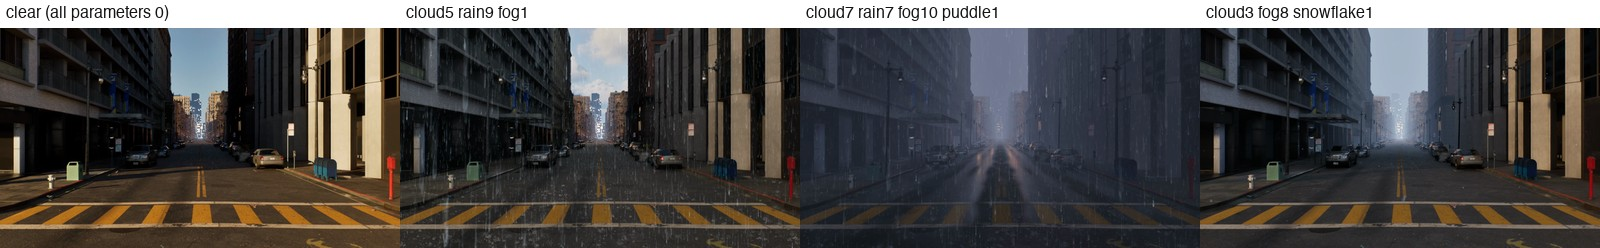
\includegraphics[width=\linewidth]{figs/fig_dataset_sim.jpg}\\[2pt]
  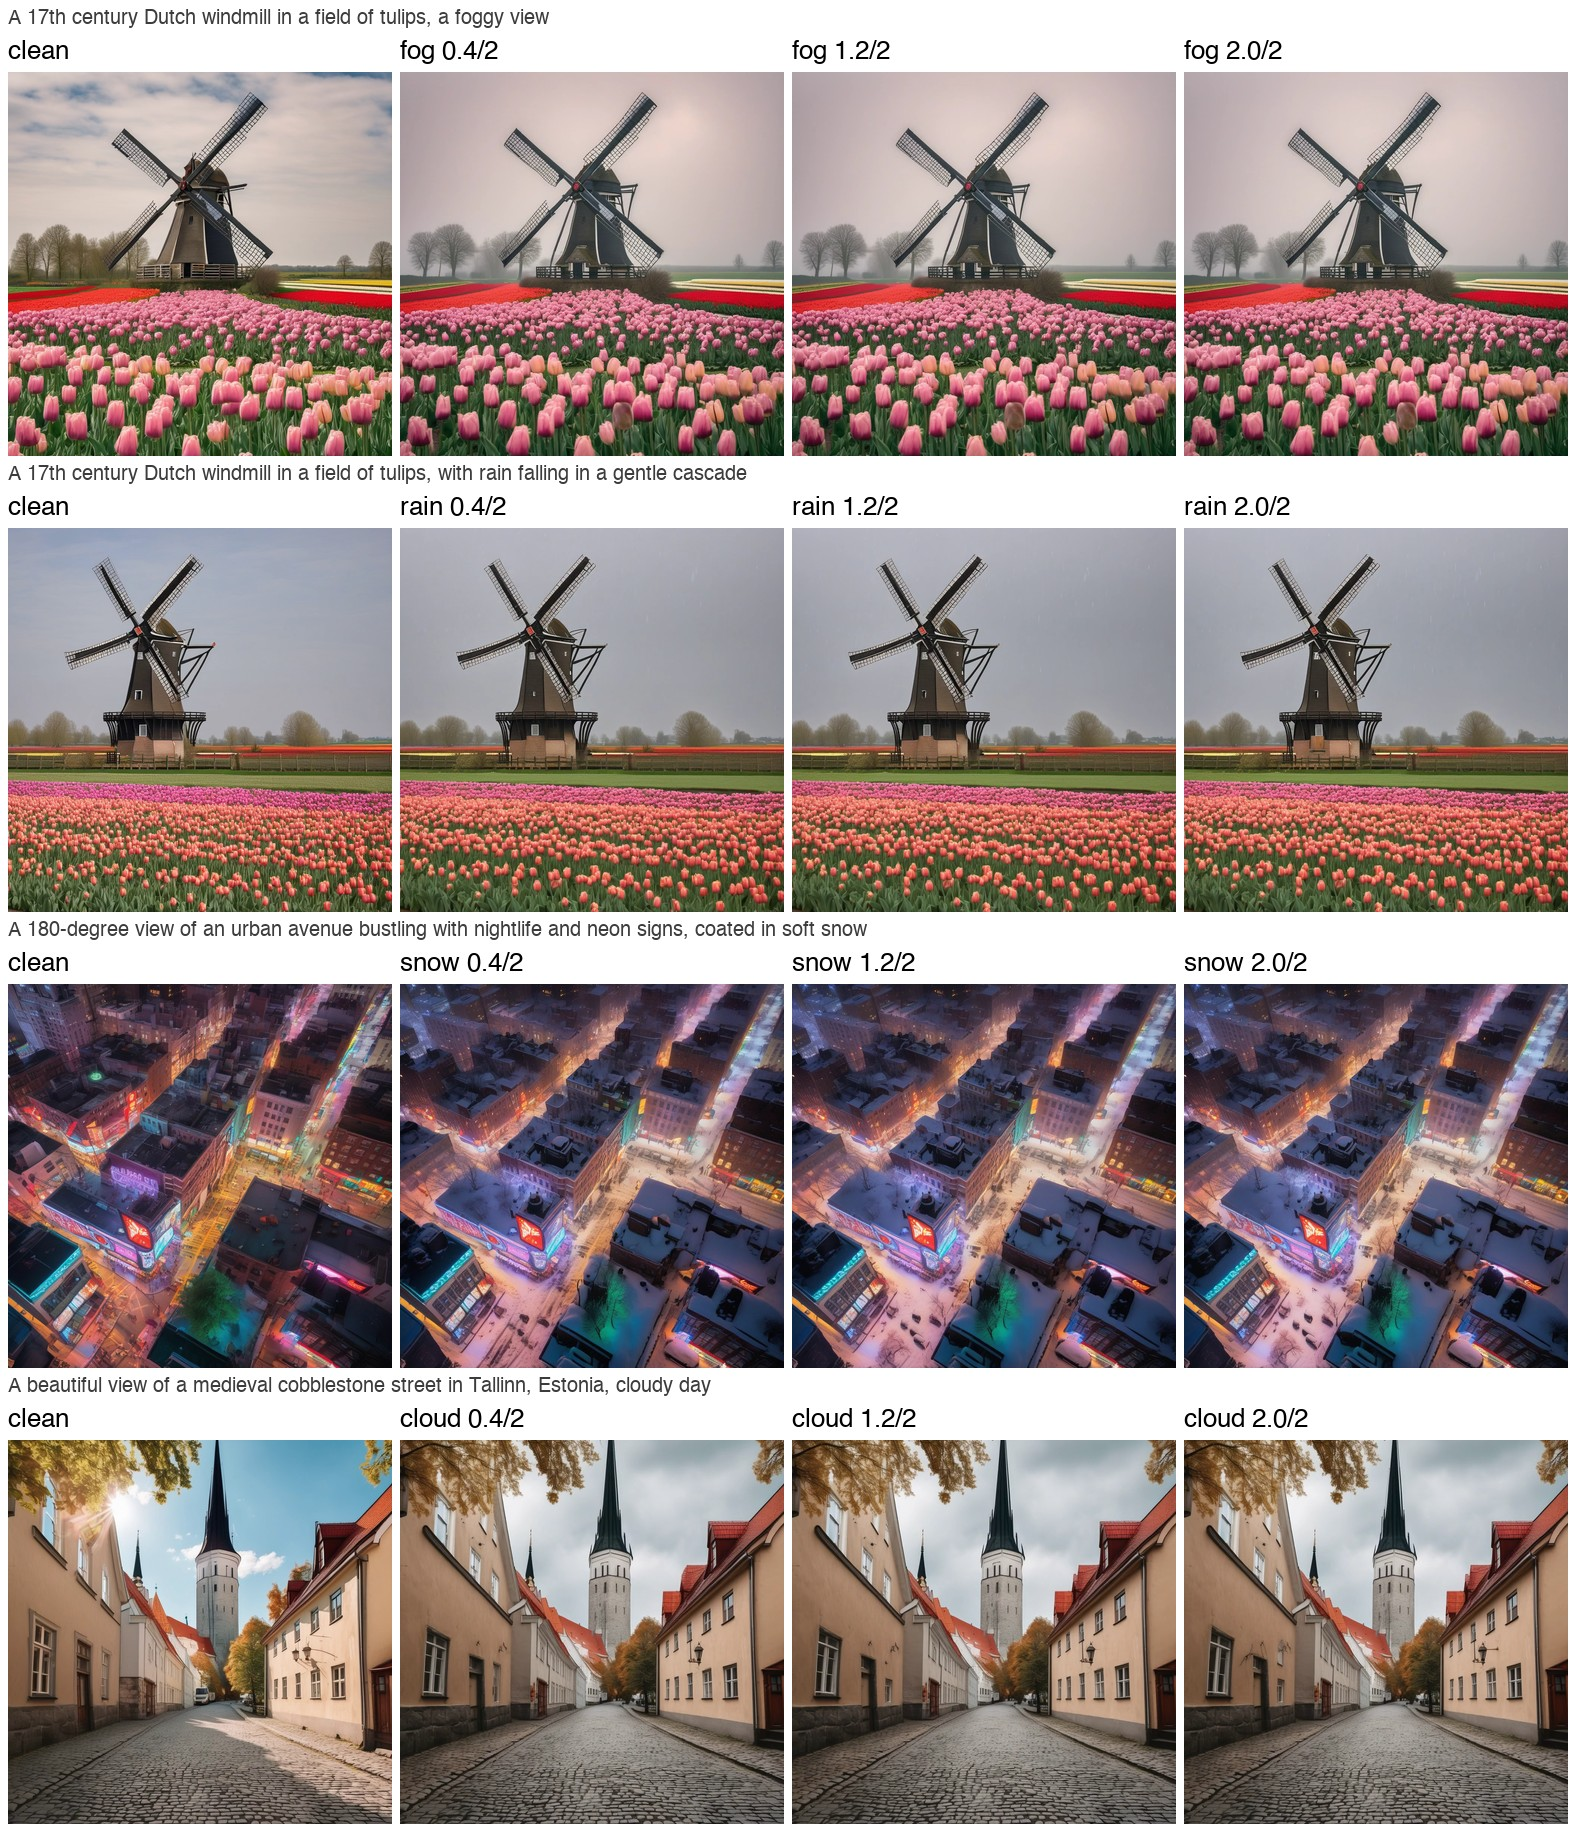
\includegraphics[width=0.62\linewidth]{figs/fig_dataset_images.jpg}
  \caption{\textbf{WeatherWeaver paired data.} Top: one simulation camera path rendered clear and under three known weather vectors (pixel-aligned). Bottom: SDXL image pairs, clean versus one weather type at increasing strength.}
  \label{fig:data}
\end{figure}

%=====================================================================
\section{Our Approach}
%=====================================================================

\subsection{Reference K/V injection}
\label{sec:kv}

\begin{figure}[!htb]
\centering
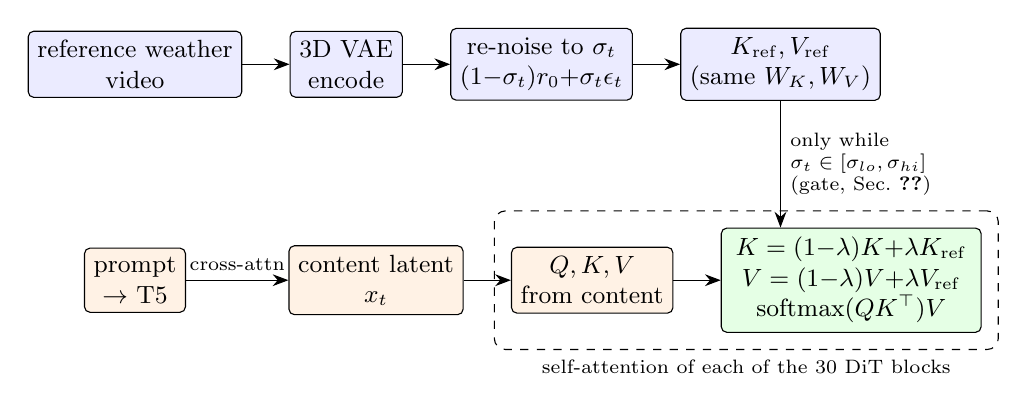
\begin{tikzpicture}[
  box/.style={draw, rounded corners=2pt, minimum height=0.8cm, align=center, font=\small, fill=#1},
  box/.default=white, >={Stealth[length=2mm]}, font=\small]
  \node[box=blue!8] (ref) {reference weather\\video};
  \node[box=blue!8, right=0.6cm of ref] (vae) {3D VAE\\encode};
  \node[box=blue!8, right=0.6cm of vae] (noise) {re-noise to $\sigma_t$\\$(1{-}\sigma_t)r_0{+}\sigma_t\epsilon_t$};
  \node[box=blue!8, right=0.6cm of noise] (kvr) {$K_{\mathrm{ref}},V_{\mathrm{ref}}$\\(same $W_K,W_V$)};
  \node[box=orange!10, below=1.9cm of ref] (txt) {prompt\\$\rightarrow$ T5};
  \node[box=orange!10, right=1.3cm of txt] (x) {content latent\\$x_t$};
  \node[box=orange!10, right=0.6cm of x] (qkv) {$Q,K,V$\\from content};
  \node[box=green!10, right=0.6cm of qkv, minimum width=3.3cm] (blend) {$K=(1{-}\lambda)K{+}\lambda K_{\mathrm{ref}}$\\$V=(1{-}\lambda)V{+}\lambda V_{\mathrm{ref}}$\\$\mathrm{softmax}(QK^\top)V$};
  \draw[->] (ref) -- (vae); \draw[->] (vae) -- (noise); \draw[->] (noise) -- (kvr);
  \draw[->] (kvr.south) -- node[right, font=\scriptsize, align=left]{only while\\$\sigma_t\in[\sigma_{lo},\sigma_{hi}]$\\(gate, Sec.~\ref{sec:gate})} (kvr.south |- blend.north);
  \draw[->] (x) -- (qkv); \draw[->] (qkv) -- (blend);
  \draw[->] (txt) -- node[above, font=\scriptsize]{cross-attn} (x);
  \node[draw, dashed, rounded corners, fit=(qkv)(blend), inner sep=6pt, label={[font=\scriptsize]below:self-attention of each of the 30 DiT blocks}] {};
\end{tikzpicture}
\caption{\textbf{Reference K/V injection.} The reference clip is encoded by the same VAE and patch embedding as the content, re-noised to the current noise level at every step, and projected by the block's own key/value weights. Queries come from the content only; keys and values are a convex blend. No new parameters are introduced.}
\label{fig:method}
\end{figure}

The reference clip is encoded with the model's own VAE and patch embedding, at the same resolution and token grid as the generated video, so reference tokens share the content's rotary positions.
At every denoising step the clean reference latent $r_0$ is re-noised to the current level with fresh noise, $r_t = (1-\sigma_t)\,r_0 + \sigma_t\,\epsilon_t$ (Eq.~\ref{eq:interp}), and passed through the same timestep modulation.
Inside the self-attention of each selected block, queries come from the content tokens only; keys and values are blended per token:
\begin{equation}
K = (1-\lam)\,K_{\mathrm{content}} + \lam\,K_{\mathrm{ref}},\qquad
V = (1-\lam)\,V_{\mathrm{content}} + \lam\,V_{\mathrm{ref}} .
\end{equation}
Injection is applied to both CFG branches (Fig.~\ref{fig:method}).
The design rests on one observation: the self-attention projections were trained on exactly this representation---noised video tokens after patch embedding and adaLN---so the reference arrives in-distribution.
An earlier design that concatenated reference features into \emph{cross}-attention (whose projections were trained on T5 text embeddings) failed for that reason.

\subsection{Paired-difference probing}
\label{sec:probe}
To ask where and when the model represents weather, we take a pixel-aligned pair (clear $x^c_0$, weather $x^w_0$), noise both with the \emph{same} $\epsilon$ to level $\sigma$, run one forward pass on each with identical (empty) conditioning, and record every block's residual output $h^c_b, h^w_b$.
Because noise, geometry, camera, frame and conditioning are identical, the difference $\Delta h_b(\sigma) = h^w_b - h^c_b$ is attributable to weather alone, and a single forward pass has no trajectory drift.
We measure: (i) the size $\|\Delta h_b\|/\|h^c_b\|$ per block and $\sigma$; (ii) whether the token-averaged difference points the same way across different scenes (cosine between pairs); (iii) the \textbf{phase}: how much of the true latent difference $x^w_0 - x^c_0$ already appears in the model's clean-image guess (Eq.~\ref{eq:x0}),
\begin{equation}
\rho(\sigma) = \frac{\|\xhat(x^w_\sigma) - \xhat(x^c_\sigma)\|}{\|x^w_0 - x^c_0\|}.
\end{equation}
The same measurement on pairs of two \emph{different clear scenes} gives a content control.
We probe 11 noise levels on the 50-step schedule (step indices 0, 5, \dots, 45, 49) and all 30 blocks.

\subsection{Exact fixed-point Euler inversion}
\label{sec:fp}
Forward noising (Sec.~\ref{sec:probe}) is a proxy for the trajectory the model actually follows.
To probe the real trajectory, we invert both members of a pair along the 50-step schedule.
Plain Euler inversion uses the velocity at the start of each step.
We instead solve the implicit backward step by fixed-point iteration,
\begin{equation}
x_{i+1}^{(k+1)} = x_i + \Delta\sigma_i\, v_\theta\!\big(x_{i+1}^{(k)},\,\sigma_{i+1}\big),\qquad x_{i+1}^{(0)} = x_i + \Delta\sigma_i\, v_\theta(x_i,\sigma_i),
\end{equation}
which at convergence is the exact inverse of the Euler sampler (ReNoise~\cite{renoise} uses the same principle).
Three iterations suffice. No gradients are involved.

\subsection{Mean-vector weather steering}
From the paired probes we average the token-mean difference $\Delta h_b(\sigma)$ over many pairs to obtain a weather direction $d_b(\sigma)$ per block and noise level.
Steering adds $\alpha\, d_b(\sigma)$ to the residual stream of selected blocks while $\sigma$ lies in a chosen window, during an ordinary generation, using forward hooks registered from outside the model (the model code is untouched).

\subsection{Window-gated injection}
\label{sec:gate}
The analysis (Sec.~\ref{sec:exp-paired}--\ref{sec:exp-ode}) says the weather is decided early.
This motivates gating the reference injection to a noise window, applying it only while $\sigma_t \in [\sigma_{lo}, \sigma_{hi}]$ (Fig.~\ref{fig:method}).
The reference noise is still drawn at every step, so the full window $[0,1]$ is identical to ungated injection.

%=====================================================================
\section{Experiments}
%=====================================================================

\paragraph{Setup.}
All generations use Wan2.2-TI2V-5B at $1280{\times}704$, 61 frames, 50 UniPC steps with shift 5, CFG 5, seed 42, on a single A100 80\,GB (IIT Bombay Param Rudra) or A40/L40S (IIT Bombay Prajna).
Analysis runs use empty text conditioning.
No model weight is modified in any experiment.

\paragraph{A note on metrics.}
Measuring weather in a generated video is itself unsolved, and we found three plausible metrics to be broken \emph{before} trusting them:
CLIP image similarity cannot detect the weather (it scores an unweathered output 0.617 and a clearly weathered one 0.616 against the reference);
the dark-channel haze prior~\cite{darkchannel} is confounded by sky and must be computed on the lower half of the frame;
and LPIPS against an un-injected baseline measures scene \emph{recomposition} rather than content loss, because injection changes the trajectory from the first step.
We therefore use (a) composition-free proxies (sky-excluded dark channel for haze, Laplacian energy for detail) for text-to-video outputs, and (b) \emph{paired ground truth} wherever the clear video is known, comparing against its real weather render.

%---------------------------------------------------------------------
\subsection{Operating point of reference injection}
\label{sec:exp-lambda}

\begin{figure}[!htb]
  \centering
  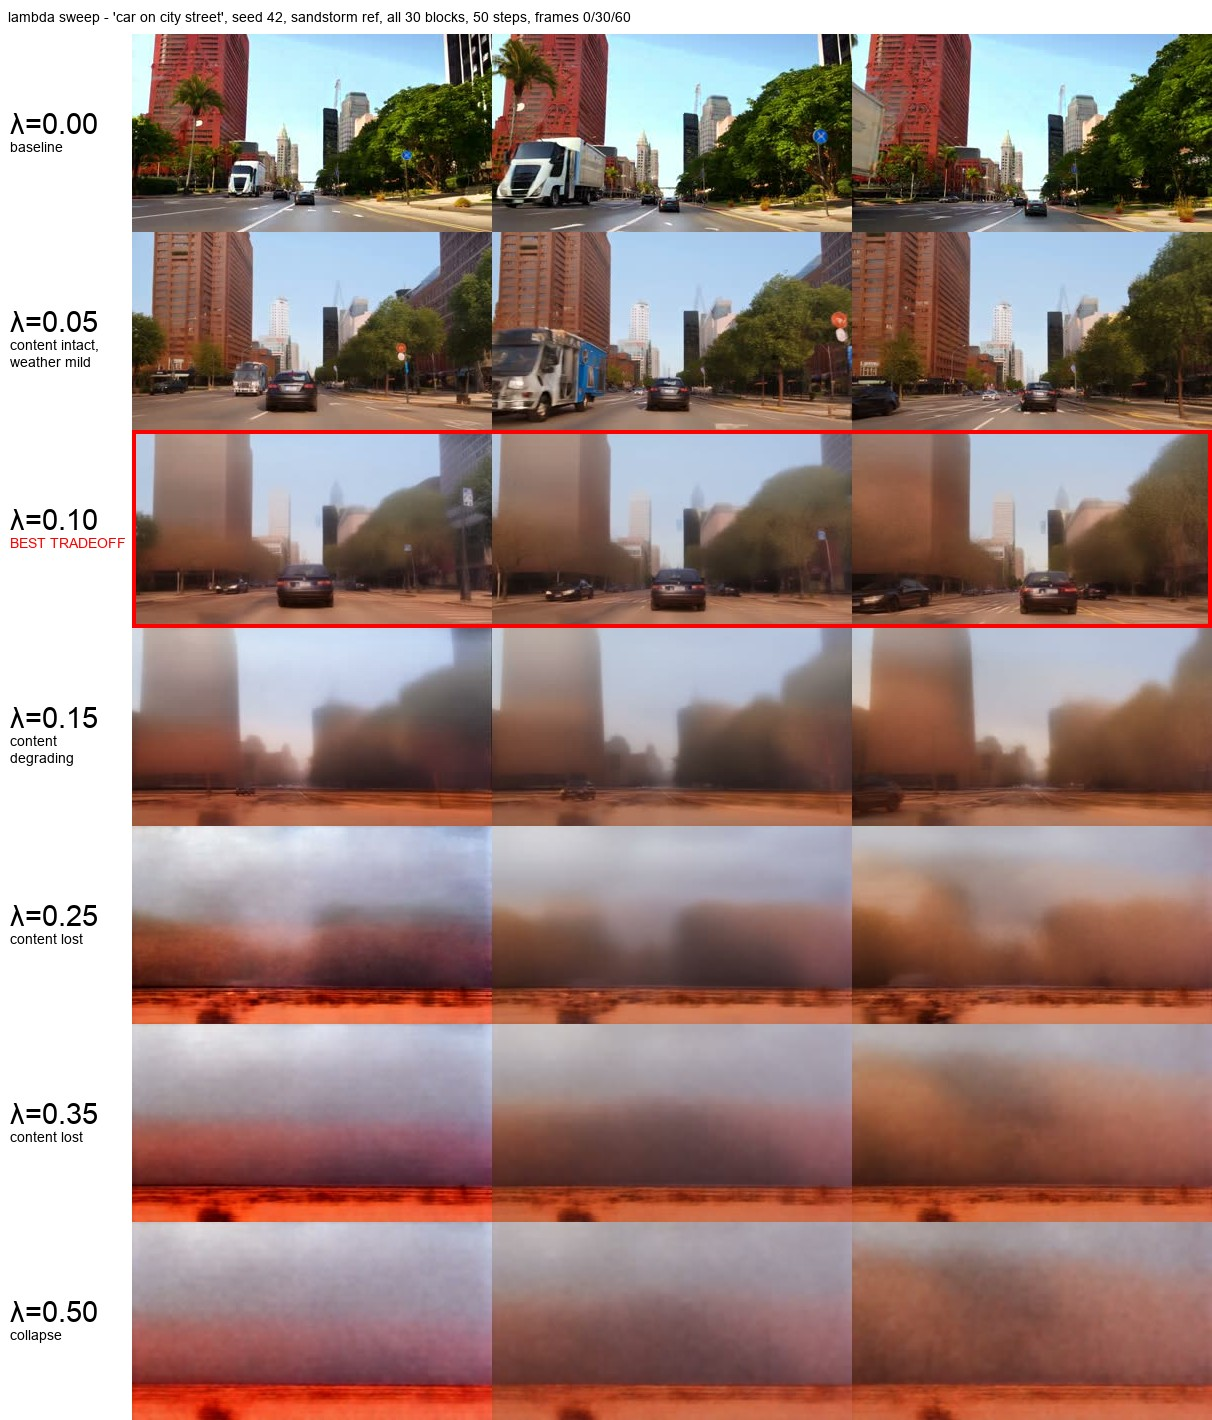
\includegraphics[width=0.55\linewidth]{figs/fig_lambda_sweep.jpg}
  \caption{\textbf{Injection strength sweep} (``car on city street'', sandstorm reference, all 30 blocks; frames 0/30/60). Degradation is progressive: $\lam{=}0.05$ keeps the scene with mild weather, $\lam{=}0.10$ applies the sandstorm while the car, road, trees and lane markings stay legible, and $\lam{\ge}0.25$ replaces the scene with the reference's own appearance.}
  \label{fig:lambda}
\end{figure}

Figure~\ref{fig:lambda} shows a seven-point sweep of $\lam$.
The earlier observation that injection ``destroys content'' (made at $\lam{=}0.5$) turns out to be an operating-point error: at $\lam{=}0.5$ the output becomes a featureless dust field because the reference's keys and values carry its \emph{scene} as well as its weather (content substitution).
At $\lam{=}0.10$ the sandstorm is clearly applied while the prompted scene survives, and this setting held across four different prompts without retuning (Fig.~\ref{fig:prompts} in the appendix).
An orange band at the bottom edge scales with $\lam$ and is essentially absent at $\lam\le 0.10$, so it is a symptom of over-injection, not an independent bug.
Injection overhead is about 1\% of generation time.

%---------------------------------------------------------------------
\subsection{Latent atlas and block ablation}
\label{sec:exp-atlas}

\begin{figure}[!htb]
  \centering
  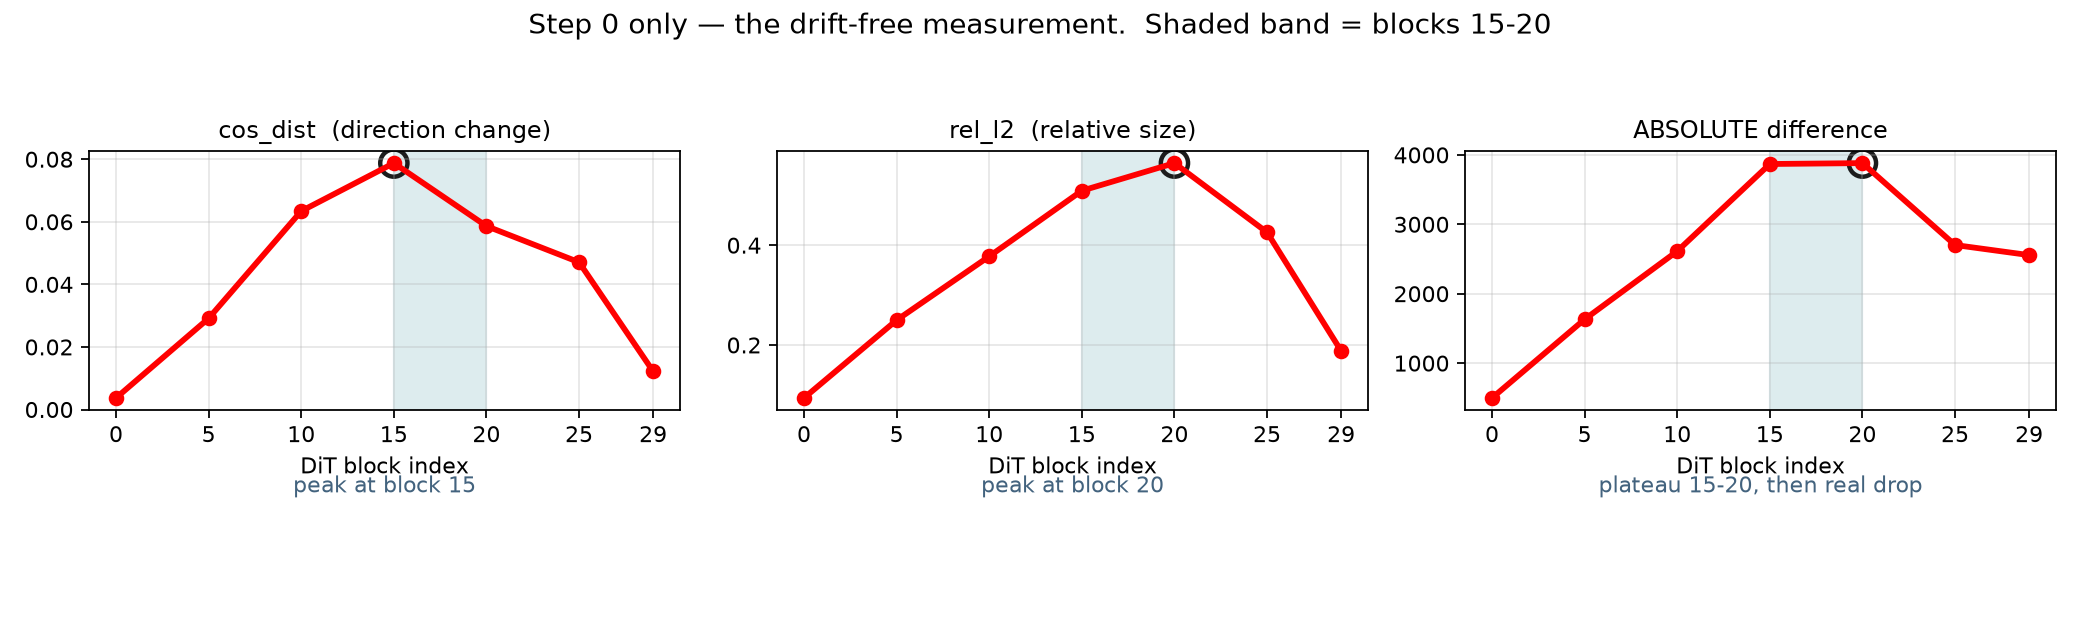
\includegraphics[width=\linewidth]{figs/fig_atlas_step0.png}
  \caption{\textbf{Where injection perturbs the network} (step 0, where injected and baseline runs share the same initial latent, so the comparison has no trajectory drift). The relative perturbation peaks at mid-depth blocks 15--20.}
  \label{fig:atlas}
\end{figure}

We captured the residual stream at 7 blocks $\times$ 14 steps for an injected and a baseline run (98 cells each).
At step 0 the perturbation peaks at \textbf{blocks 15--20} (Fig.~\ref{fig:atlas}).
Ratio metrics initially suggested the last block ``absorbs'' the injection, but block 29 doubles the residual norm; in absolute terms it keeps about 66\% of the peak perturbation (absolute difference 3882 at block 20 versus 2556 at block 29).
We then injected into block subsets only (from the last block alone up to the last 11 blocks), at matched and at higher $\lam$: \textbf{no subset of up to 11 blocks produced depth-structured weather}---only tint and blur---while all 30 blocks did (Fig.~\ref{fig:subsets} in the appendix).
Weather in this model is therefore not a property of a few late ``style'' blocks.

%---------------------------------------------------------------------
\subsection{Does inverting the reference help?}
\label{sec:exp-inv}

StyleID~\cite{styleid} spends 66\% of its runtime DDIM-inverting the style image and harvests keys and values along the inversion trajectory.
We replaced forward re-noising with the PreciseInv~\cite{preciseinv} solution.
Its rectified-flow formulation matches Wan2.2 exactly ($x_0 = x_\sigma - \sigma v$), so the feared incompatibility of flow matching with inversion was not an obstacle.
We solved all 50 subproblems on our own schedule (0.59\,h on an A100, mean 8.8 iterations per step; warm-starting each subproblem from the previous solution cut iterations about $10\times$ relative to the paper's random initialisation), and the inversion reconstructs the reference 3.85$\times$ better than a random draw.
Activation checkpointing was mandatory: naive backpropagation through the 5B model ran out of memory at 77\,GB, versus 19\,GB with per-block checkpointing.

\begin{figure}[!htb]
  \centering
  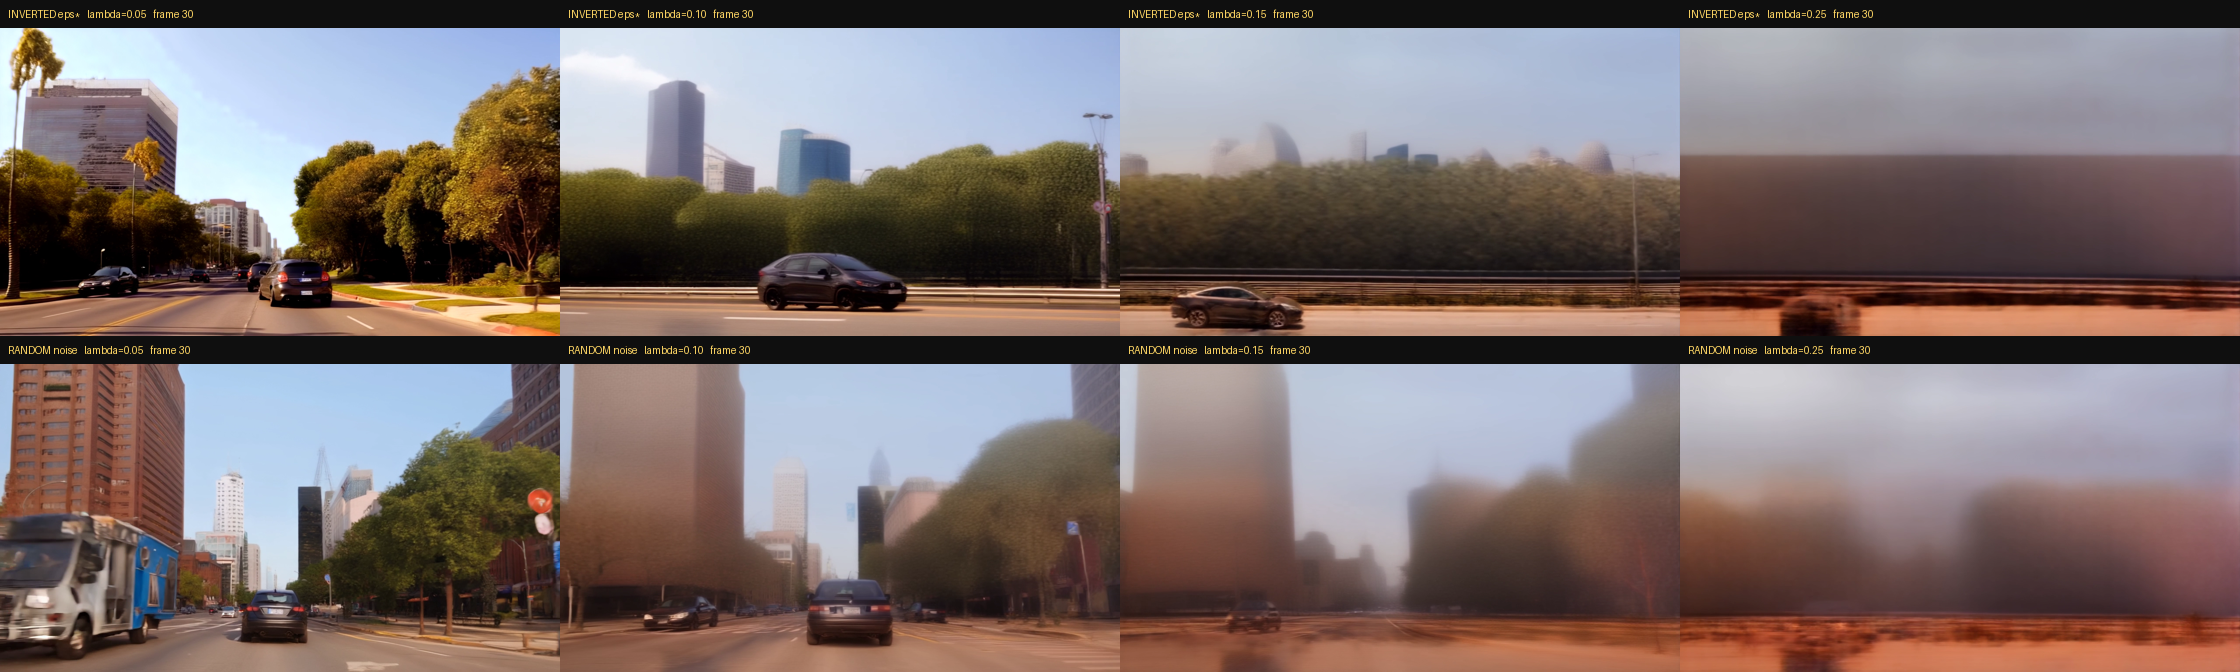
\includegraphics[width=\linewidth]{figs/fig_inv_ladder.png}
  \caption{\textbf{Inverted (top) versus random (bottom) reference noise} at matched $\lam\in\{0.05,0.10,0.15,0.25\}$. Inversion gives a clear sky at $\lam\le0.10$ and collapses at 0.25; random re-noising gives depth-structured dust.}
  \label{fig:invladder}
\end{figure}

\begin{table}[!htb]
\centering\small
\begin{tabular}{lcccc|c}
\toprule
$\lam$ & 0.05 & 0.10 & 0.15 & 0.25 & reference \\
\midrule
haze, random re-noising $\uparrow$ & 0.177 & \textbf{0.203} & 0.213 & 0.198 & \multirow{2}{*}{0.286} \\
haze, inverted reference  & 0.107 & 0.113 & 0.135 & 0.178 & \\
\midrule
detail, random re-noising & 0.040 & 0.025 & 0.016 & 0.015 & \multirow{2}{*}{0.009} \\
detail, inverted reference & 0.066 & 0.040 & 0.048 & 0.019 & \\
\bottomrule
\end{tabular}
\caption{\textbf{Inversion makes transfer strictly worse.} Haze = dark-channel prior on the sky-free lower half; detail = Laplacian energy. Random re-noising at $\lam{=}0.05$ already gives as much haze as the inverted reference at $\lam{=}0.25$, with 2.2$\times$ the detail.}
\label{tab:inv}
\end{table}

\textbf{Result: negative.} At every $\lam$, random re-noising dominates (Table~\ref{tab:inv}, Fig.~\ref{fig:invladder}); every inverted point lies on or inside the random-noise Pareto frontier.
Diagnosis: the 50 solved noises are essentially \emph{one direction} (consecutive cosine 1.000; first-to-last 0.84, versus 0.0006 for independent Gaussians), whereas the random path draws 50 independent noises whose noise components average out.
Our interpretation is that forward re-noising is the training-time noising formula and therefore in-distribution at every $\sigma$, while an approximate inversion trajectory is on neither the data nor the training manifold.
One confound remains: the inversion was solved without CFG and deployed with CFG~5.

%---------------------------------------------------------------------
\subsection{Paired-data analysis: where and when is weather represented?}
\label{sec:exp-paired}

We ran the paired probe (Sec.~\ref{sec:probe}) on \textbf{167 clear/weather pairs} from about ten camera paths in each of the four Unreal worlds, plus 20 content-control pairs (two different clear scenes) and \textbf{60 single-factor image pairs} (10 per weather type, panoramic and aerial prompts excluded).

\paragraph{When: weather is committed before content.}
Figure~\ref{fig:phase} plots the phase measure $\rho(\sigma)$.
In \textbf{every world}, the model's clean-image guess contains more of the weather difference than of a scene difference at high noise: at $\sigma{=}0.95$ it has committed 0.42 of the weather difference versus 0.19 of the scene difference in the city world (0.38/0.30, 0.35/0.22 and 0.47/0.26 in the other three).
In the town and bush-road worlds the two curves meet by $\sigma\approx0.85$--$0.88$; in the city and rural worlds the weather stays ahead until $\sigma\approx0.6$. The window in which weather leads in \emph{every} world is therefore $\sigma\approx0.92$--$0.98$, about steps 5--15 of 50.
The image pairs reproduce the weather curve (0.21/0.33/0.42 at $\sigma$ 0.98/0.95/0.92).
This is consistent with diffusion's known coarse-to-fine order---weather here is mostly low-frequency light and haze---so we present it as a measured property of weather in this model rather than a new mechanism.

\begin{figure}[!htb]
  \centering
  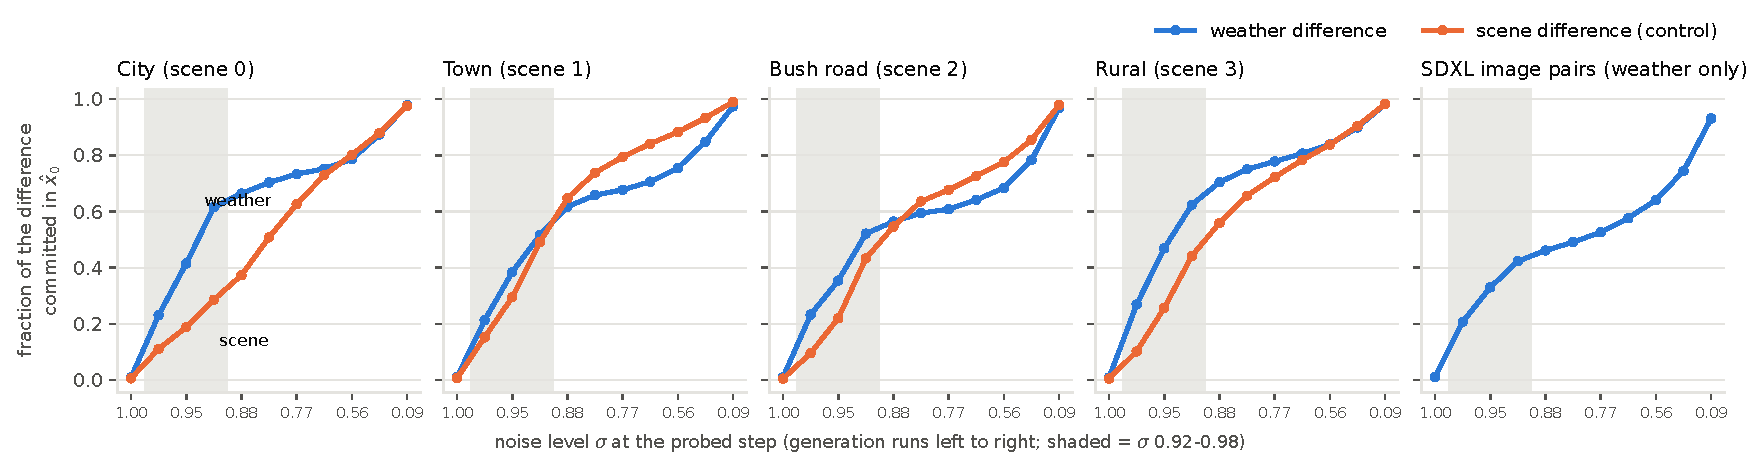
\includegraphics[width=\linewidth]{figs/fig_phase_worlds.pdf}
  \caption{\textbf{Weather is committed before scene content in all four worlds.} Fraction of the true latent difference already present in the model's clean-image guess $\xhat$ at each noise level, for clear$\to$weather pairs (blue) and for pairs of two different clear scenes (orange). Shaded: $\sigma$ 0.92--0.98.}
  \label{fig:phase}
\end{figure}

\paragraph{Where: a generic magnitude peak, a specific type signal.}
The raw size of the weather difference is amplified most at \textbf{block 22} (up to $7.4\times$ the input difference at $\sigma{=}0.95$; Fig.~\ref{fig:where}, appendix), but the content control shows the same block-22 peak ($5$--$6\times$), so that peak is a property of the network, not of weather.
What \emph{is} weather-specific is the signal that distinguishes weather families: the same-family minus cross-family cosine peaks at \textbf{blocks 19--22 for $\sigma$ 0.83--0.92} (up to $+0.31$), inside the phase window and consistent with the mid-depth peak of Sec.~\ref{sec:exp-atlas}.

\paragraph{Disentanglement: is there a content-independent weather direction?}
Within one world, the token-mean weather difference points the same way across different camera paths (cosine 0.5--0.8 for $\sigma\le0.95$), while scene differences do not ($-0.1$ to $-0.2$; random 3072-d vectors: $0\pm0.018$).
\textbf{Across worlds the shared direction is real but much weaker} (Fig.~\ref{fig:crossenv}): 0.05--0.40 at blocks 19--22 against a control of $\approx0.01$, highest at low noise (0.58 at block 22, $\sigma{=}0.09$) and nearly absent at blocks 19--22 inside the high-noise window, where early blocks (1--11) carry more (0.15--0.25).
We report this correction explicitly: our single-world result overstated how general the weather direction is.

\begin{figure}[!htb]
  \centering
  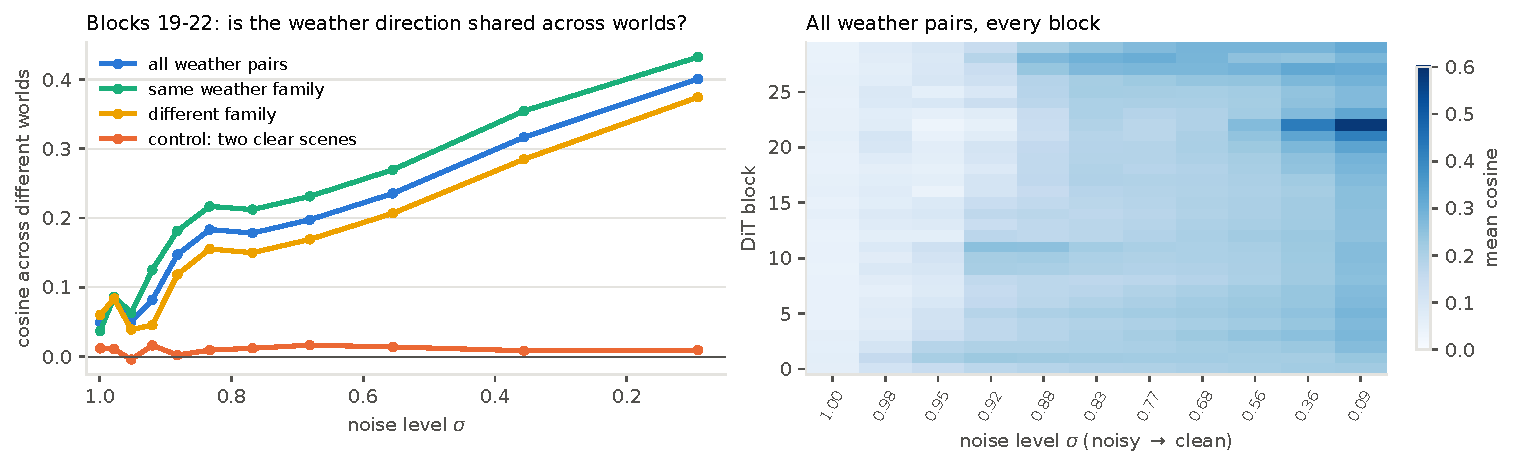
\includegraphics[width=\linewidth]{figs/fig_cross_env.pdf}
  \caption{\textbf{Cross-world consistency of the weather direction} (167 pairs, four worlds). Left: cosine between token-mean weather differences of pairs from \emph{different} worlds, blocks 19--22; the two-clear-scenes control stays at zero. Right: the same for every block.}
  \label{fig:crossenv}
\end{figure}

\paragraph{Weather type is decodable.}
On the single-factor image pairs, a leave-one-out nearest-centroid classifier on the token-mean difference identifies the weather type with up to \textbf{91.7\% accuracy} (chance 16.7\%), best at blocks 3--10 over most noise levels (Fig.~\ref{fig:types}).
After block 0 the accuracy is already 60--77\%, so much of the type information is present in the input, and the early blocks sharpen it by 15--20 points.
Snow and snowflake are similar to the model (cosine 0.62); cloud and rain are the least self-consistent, matching how faint those edits are in the data.
The classifier fits only class means, so this is a training-free probe.

\begin{figure}[!htb]
  \centering
  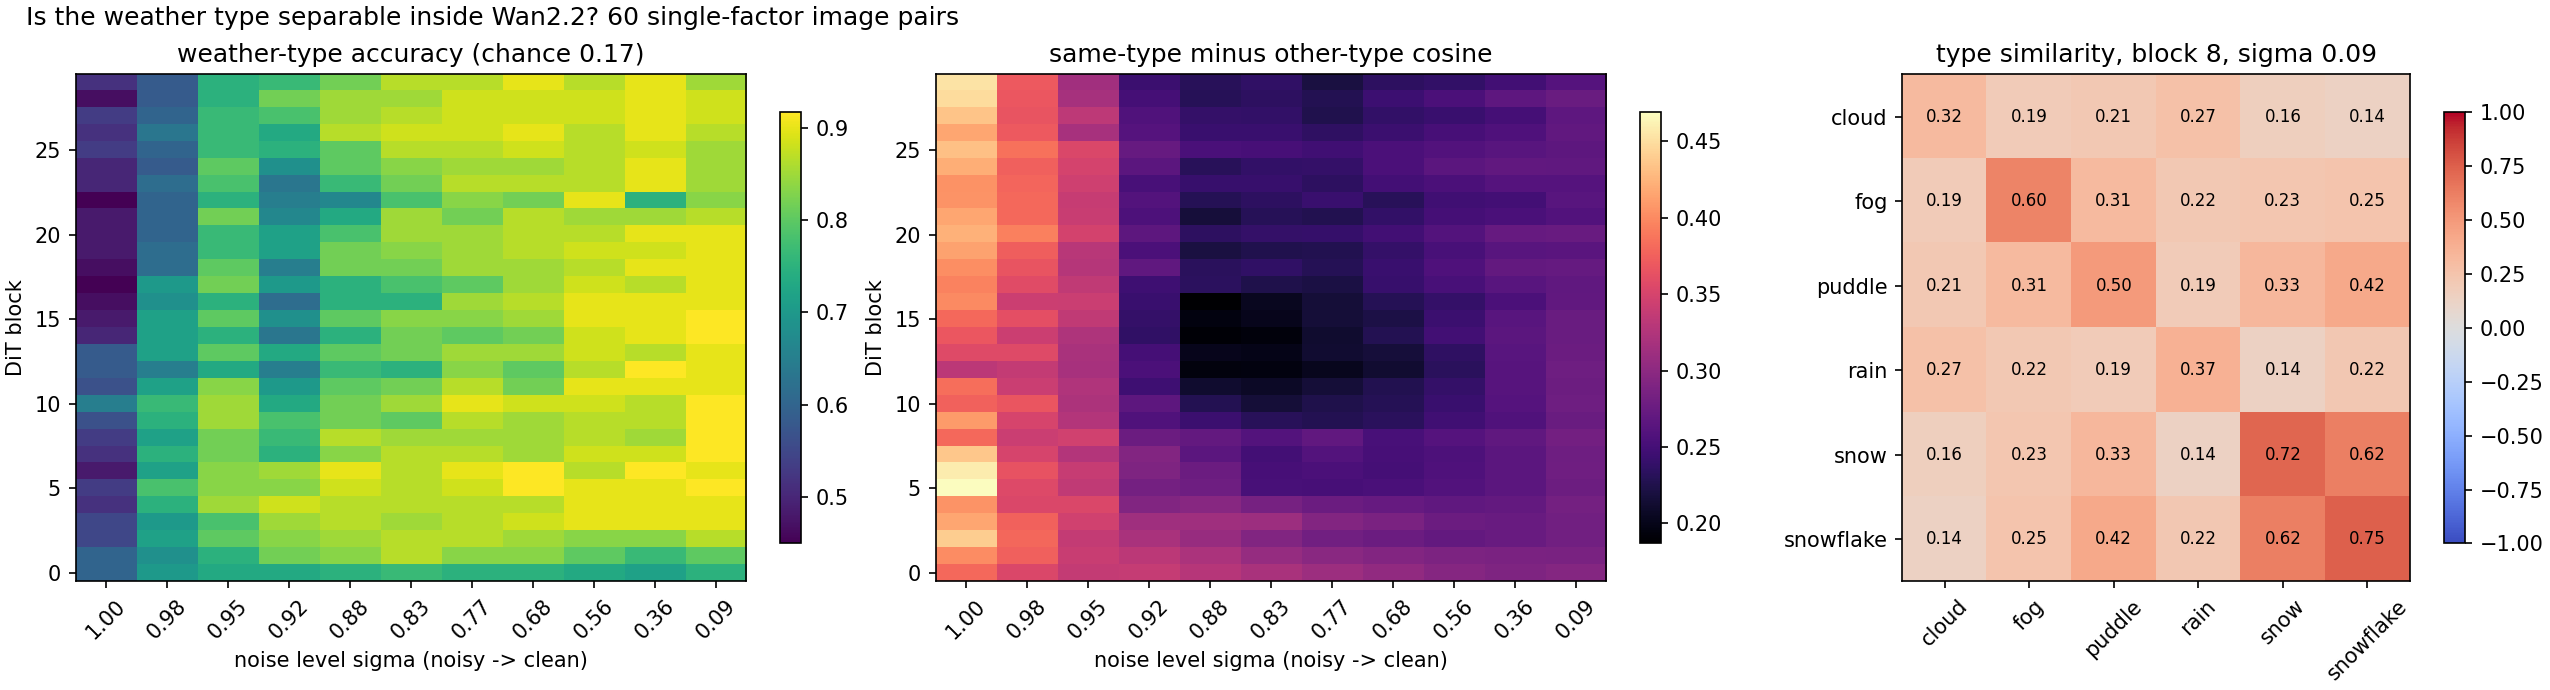
\includegraphics[width=\linewidth]{figs/fig_types.png}
  \caption{\textbf{The weather type can be read from Wan2.2's residual stream.} Left: leave-one-out nearest-centroid accuracy per block and noise level (chance 0.17). Middle: same-type minus other-type cosine. Right: type-similarity matrix at the best cell.}
  \label{fig:types}
\end{figure}

%---------------------------------------------------------------------
\subsection{Exact inversion: when is the weather locked in?}
\label{sec:exp-ode}

The supervisor asked whether \emph{inversion} reveals a phase in which style and content separate.
We inverted both members of clear/weather pairs with plain Euler (8 pairs) and with the fixed-point inversion of Sec.~\ref{sec:fp} (4 pairs).
\textbf{Reconstruction improves from 0.43/0.58 to 0.042/0.102 relative error} (clear/weather) with three fixed-point iterations, so the inverted trajectories are faithful.

\begin{figure}[!htb]
  \centering
  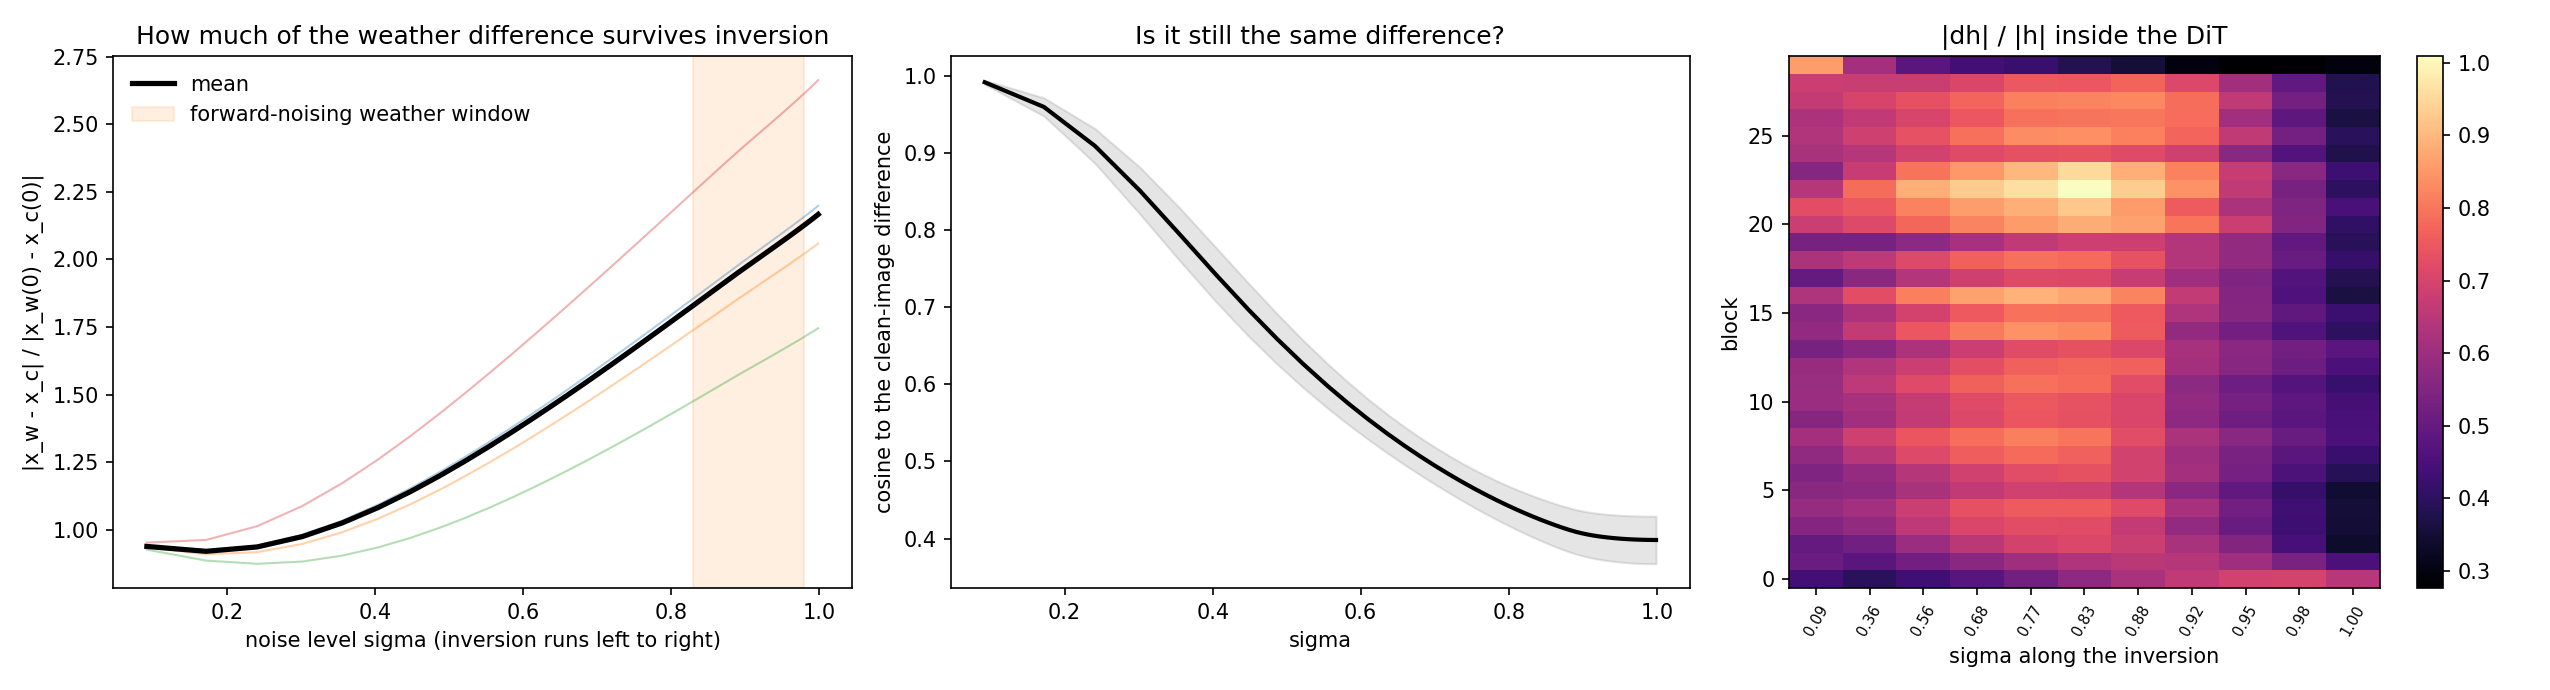
\includegraphics[width=\linewidth]{figs/fig_inversion.png}
  \caption{\textbf{Exact inversion of clear/weather pairs.} Left: size of the latent weather difference along the inversion, relative to the clean difference. Middle: its direction relative to the clean difference---it rotates between $\sigma\approx0.2$ and $0.85$ and then stops changing: the weather is locked into the noise by $\sigma\approx0.9$. Right: the difference inside the DiT, largest at blocks $\sim$20--23 for $\sigma$ 0.68--0.88.}
  \label{fig:ode}
\end{figure}

Three findings (Fig.~\ref{fig:ode}):
\begin{enumerate}
  \item \textbf{The weather is never erased; it is transformed and then locked in.} The latent weather difference grows to $2.17\times$ its clean size at $\sigma{=}1$; its direction rotates away from the pixel-space difference (cosine 0.99 at $\sigma{=}0.1$, 0.74 at 0.4, 0.44 at 0.8) and then \textbf{plateaus at $\approx0.40$ from $\sigma\approx0.9$ to 1}.
  \item \textbf{The weather lives in the noise.} The clear and weather videos invert to noises with cosine $0.27\pm0.13$ (independent noises: $\approx0$), and regenerating from them restores the full weather difference (ratio 1.02).
  \item \textbf{Forward-noising probes are faithful except at the highest noise.} The weather direction along the true trajectory agrees with the forward-noising probe at cosine $\ge0.9$ for $\sigma\le0.68$, but only 0.27--0.49 for $\sigma\ge0.92$.
\end{enumerate}
Together with Sec.~\ref{sec:exp-paired}: \emph{yes}, there is a phase---the weather is decided in the first few steps (high noise), before the scene content.

%---------------------------------------------------------------------
\subsection{Using the analysis (1): mean-vector steering}
\label{sec:exp-steer}

We built weather directions from 36--40 scene-0 pairs (leave-one-path-out stability: cosine 0.98--1.00) and added them to blocks 19--22 inside the weather window.

\paragraph{Paired ground-truth evaluation.}
For a clear video we know what its weather version should look like, so we evaluate against it.
A first protocol (re-noise the clear video to $\sigma{=}0.95$ and denoise) was invalid: even the unsteered arm became a featureless blur.
We therefore invert the clear video exactly (Sec.~\ref{sec:fp}), which reconstructs it at 3.7--4.2\% error, and regenerate it with and without steering.
We report the fraction of the true weather difference realised along its direction (frac), the cosine between the change and the true difference (cos), and the distance to the real weather render relative to the unsteered regeneration (err; $<1$ means closer than doing nothing).

\begin{table}[!htb]
\centering\small
\begin{tabular}{lccccc}
\toprule
arm (blocks 19--22) & frac & cos & err $\downarrow$ & PSNR vs.\ weather $\uparrow$ & runs with err$<1$ \\
\midrule
no steering & 0 & -- & 1.00 & 17.9 & -- \\
$\alpha{=}1$, $\sigma$ 0.83--0.95 & 0.30 & 0.22 & 1.62 & 9.9 & 0/10 \\
$\alpha{=}1$, $\sigma$ 0.55--0.92 & 0.49 & 0.30 & 1.72 & 9.4 & 0/10 \\
$\alpha{=}2$, $\sigma$ 0.55--0.92 & 0.64 & 0.31 & 2.12 & 5.3 & 0/10 \\
$\alpha{=}4$, $\sigma$ 0.83--0.95 & 0.37 & 0.21 & 1.92 & 5.8 & 0/10 \\
weather-matched dir., $\alpha{=}0.5$ & 0.37 & 0.32 & 1.25 & 14.8 & 1/4 \\
\bottomrule
\end{tabular}
\caption{\textbf{Steering points the right way but lands further from the real weather.} Ten scene-0 pairs, exact-inversion baseline. Adding blocks 1--10 or all 30 blocks raised frac to 1.08 but err to 1.87--2.51.}
\label{tab:steer}
\end{table}

\begin{figure}[!htb]
  \centering
  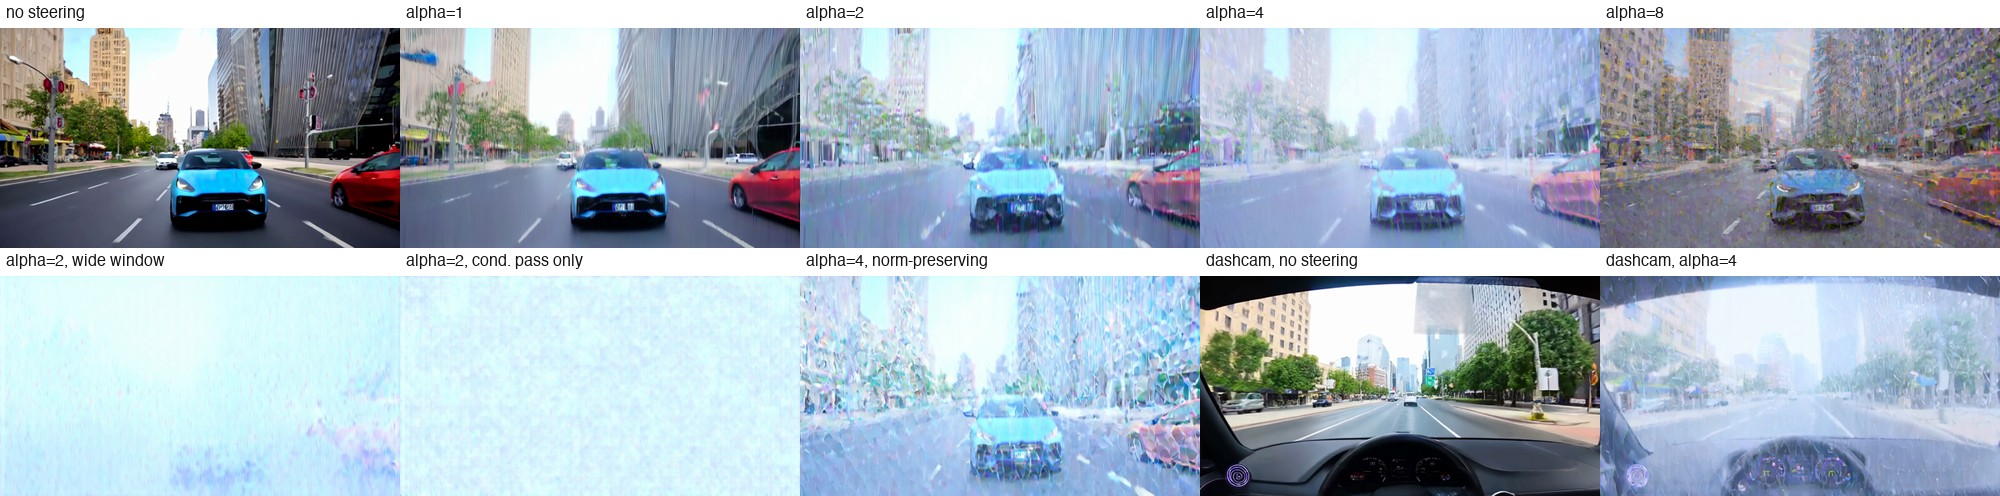
\includegraphics[width=\linewidth]{figs/fig_steer_sweep.jpg}
  \caption{\textbf{Text-to-video steering sweep} (same seed). Only $\alpha\approx1$ is usable: it keeps the composition exactly and adds haze and streaks. Stronger or wider steering produces speckle, a white field, or a shattered-glass mosaic.}
  \label{fig:steer}
\end{figure}

\textbf{Result: negative} (Table~\ref{tab:steer}, Fig.~\ref{fig:steer}).
Steering always moves the video \emph{along} the true weather difference (frac 0.30--1.08), but always lands further from the real render than doing nothing.
In text-to-video it preserves the composition exactly---a real advantage---but adds a bright bluish veil and streaks rather than the darkening of real bad weather.
Diagnosis: a token-mean direction adds the same vector at every position, whereas weather is spatially structured (sky versus road, near versus far); a cosine of 0.2--0.4 with the true difference means most of the push is off-axis.
Attention-based injection is spatially adaptive by construction, which motivates returning to it.

%---------------------------------------------------------------------
\subsection{Using the analysis (2): window-gated injection}
\label{sec:exp-gated}

If the weather is decided in the first steps, injecting the reference only there should carry most of the effect, and injecting only later should carry little.

\begin{figure}[!htb]
  \centering
  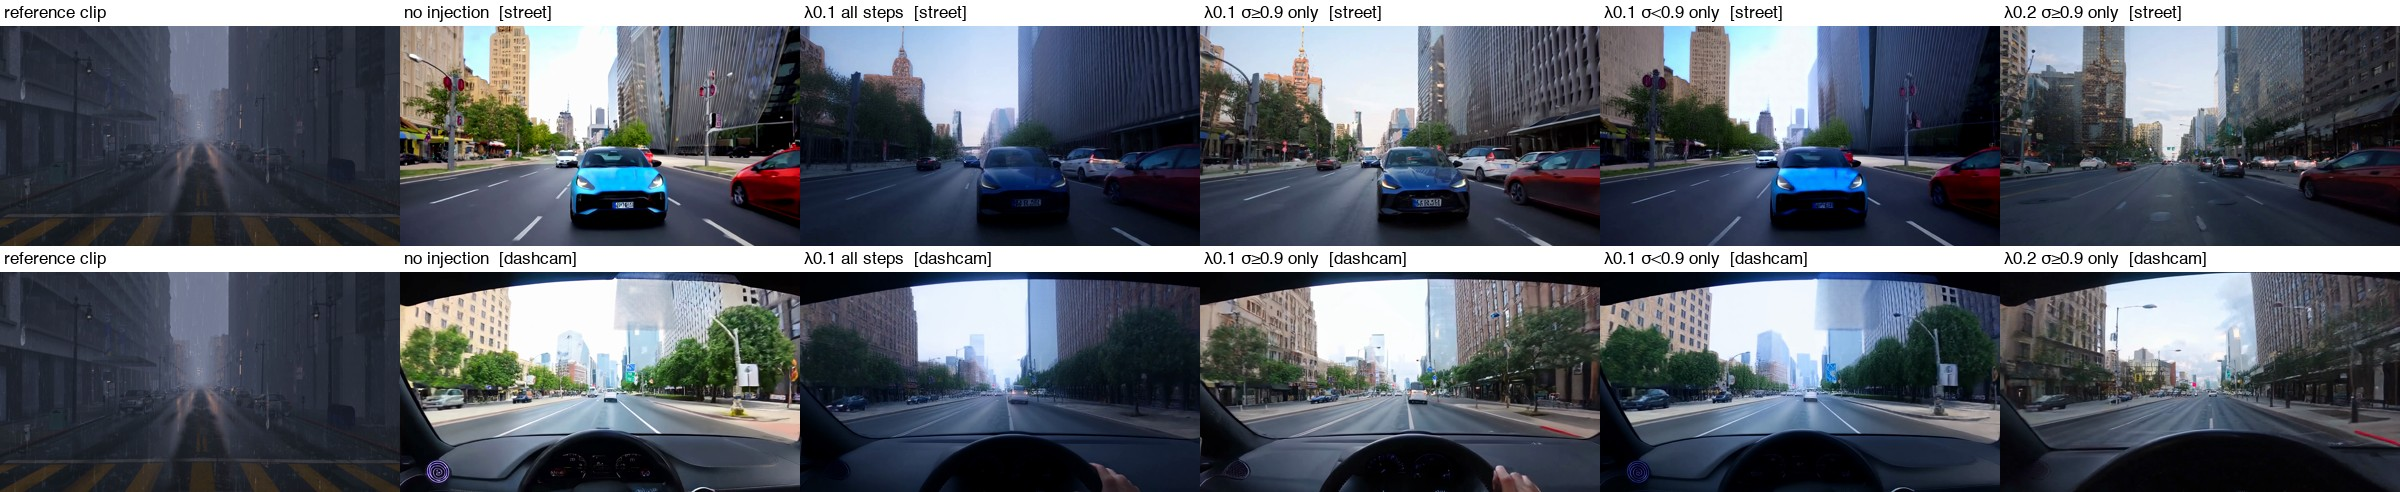
\includegraphics[width=\linewidth]{figs/fig_gated_sheet.jpg}
  \caption{\textbf{Window-gated injection} (first-person rain/fog reference from WeatherWeaver, same seed, $\lam{=}0.1$ unless noted). Early-only injection ($\sigma\ge0.9$) gives most of the all-steps effect---darker, overcast light---while late-only injection ($\sigma<0.9$) is almost identical to no injection. Rows: two prompts.}
  \label{fig:gated}
\end{figure}

\paragraph{Text-to-video.}
Figure~\ref{fig:gated} confirms the prediction with a first-person heavy-rain/fog reference and a dashcam prompt: \textbf{early-only injection reproduces most of the all-steps effect, late-only injection does almost nothing}.
Two limitations are visible: the early steps also set the layout, so early injection re-composes the scene (at $\lam{=}0.2$ the car disappears); and no arm transfers the reference's rain streaks or fog density---the transfer is mostly of light and atmosphere.

\paragraph{Paired ground truth.}
We evaluate gated injection exactly as steering, with one safeguard against leakage: the reference for each held-out pair is the weather render of a \emph{different} camera path with the nearest weather vector, so it can transfer weather but not the target's scene.

% PARTIAL: the 4 weather variants of scene-0 path 0000 (Param Rudra job 496461, 2026-11-19); paths 0001/0002 still running.
% Regenerate:  python3 summarize_evkv.py <metrics dir> > report/tables/kv_eval.tex
% 4 pairs from ['0000']; generated by summarize_evkv.py
\begin{table}[!htb]
\centering\small
\begin{tabular}{lcccccc}
\toprule
arm & frac & cos & err$\downarrow$ & W$\uparrow$ & C$\uparrow$ & err$<1$ \\
\midrule
no injection & 0.00 & 0.00 & 1.00 & 15.8 & 42.9 & --/4 \\
$\lambda{=}0.1$, $\sigma<0.9$ & 0.38 & 0.40 & 1.09 & 17.4 & 14.2 & 1/4 \\
$\lambda{=}0.1$, all steps & 0.58 & 0.49 & 1.14 & 16.2 & 12.0 & 1/4 \\
$\lambda{=}0.1$, $\sigma\ge0.8$ & 0.36 & 0.49 & 0.94 & 19.1 & 15.0 & 3/4 \\
$\lambda{=}0.1$, $\sigma\ge0.9$ & 0.22 & 0.45 & 0.90 & 18.7 & 19.8 & 4/4 \\
$\lambda{=}0.2$, $\sigma<0.9$ & 0.67 & 0.46 & 1.38 & 14.6 & 10.8 & 0/4 \\
$\lambda{=}0.2$, all steps & 0.84 & 0.50 & 1.51 & 14.5 & 10.6 & 0/4 \\
$\lambda{=}0.2$, $\sigma\ge0.8$ & 0.56 & 0.52 & 1.05 & 17.1 & 12.5 & 2/4 \\
$\lambda{=}0.2$, $\sigma\ge0.9$ & 0.37 & 0.47 & 0.97 & 18.6 & 15.7 & 3/4 \\
\bottomrule
\end{tabular}
\caption{\textbf{Paired ground-truth evaluation of reference injection} (4 held-out scene-0 pairs, means). frac: fraction of the true weather difference realised along its direction; cos: cosine of the change with the true difference; err: distance to the real weather render relative to the un-injected regeneration (${<}1$ = closer); W / C: PSNR (dB) to the real weather render / to the clear video. References are weather renders of a \emph{different} camera path with the nearest weather vector.}
\label{tab:kv}
\end{table}


\textbf{Preliminary result} (Table~\ref{tab:kv}): unlike steering, reference injection lands \emph{closer} to the real weather render than the unsteered regeneration in two of three pairs, and \textbf{the early window gives the best trade-off}: as much or more weather than all-step injection while preserving far more of the scene (PSNR to the clear video 20--29\,dB versus 12--20\,dB at $\lam{=}0.1$).
The failing pair is instructive: its nearest reference had weaker weather than the target.

%=====================================================================
\section{Conclusion and Future Work}
%=====================================================================

We set out to make a frozen video model render weather from an example, and ended up mapping when and where the model decides the weather.
The answers are consistent across three probes, four simulated worlds and an image set: \textbf{Wan2.2 commits to the weather in the first, highest-noise steps, before it commits to the scene}; an exact inversion shows the weather locked into the noise by $\sigma\approx0.9$; and the weather type is linearly readable in the residual stream.
Practically, reference K/V injection at $\lam{=}0.10$ is a working training-free method, and gating it to the early window carries most of its effect.
Two intuitive improvements---inverting the reference and steering along a mean weather direction---did not help, and we explained why.

\paragraph{Limitations.}
(i) All paired data is synthetic (Unreal renders, SDXL edits); no real weather footage was evaluated.
(ii) Transfer is mostly of light and atmosphere; heavy rain and snow texture do not carry over at content-preserving strengths.
(iii) Early injection also influences layout, so gating does not by itself protect content in text-to-video.
(iv) The ground-truth evaluation of gated injection covers a small number of pairs in one world.
(v) There is still no reliable automatic metric for weather in generated video without paired ground truth.

\paragraph{Future work.}
\begin{itemize}
  \item \textbf{Spatially adaptive steering}: replace the single mean vector by per-token directions (e.g.\ predicted from content tokens), which our diagnosis suggests is what steering lacks.
  \item \textbf{Separate the layout and weather windows}: our phase curves show weather leads content only in a narrow band; combining early weak injection with a content anchor (e.g.\ attention from an unweathered pass) may keep the scene fixed.
  \item \textbf{Cross-world and real-data evaluation} of gated injection, and inversion under CFG to remove the remaining confound of the inversion experiment.
  \item \textbf{Weather estimation}: use the decodable type and intensity signal to estimate weather parameters from a reference clip and inject them, rather than raw appearance.
\end{itemize}

\bibliographystyle{plain}
\bibliography{refs}

\appendix
\section{Additional figures}

\begin{figure}[!htb]
  \centering
  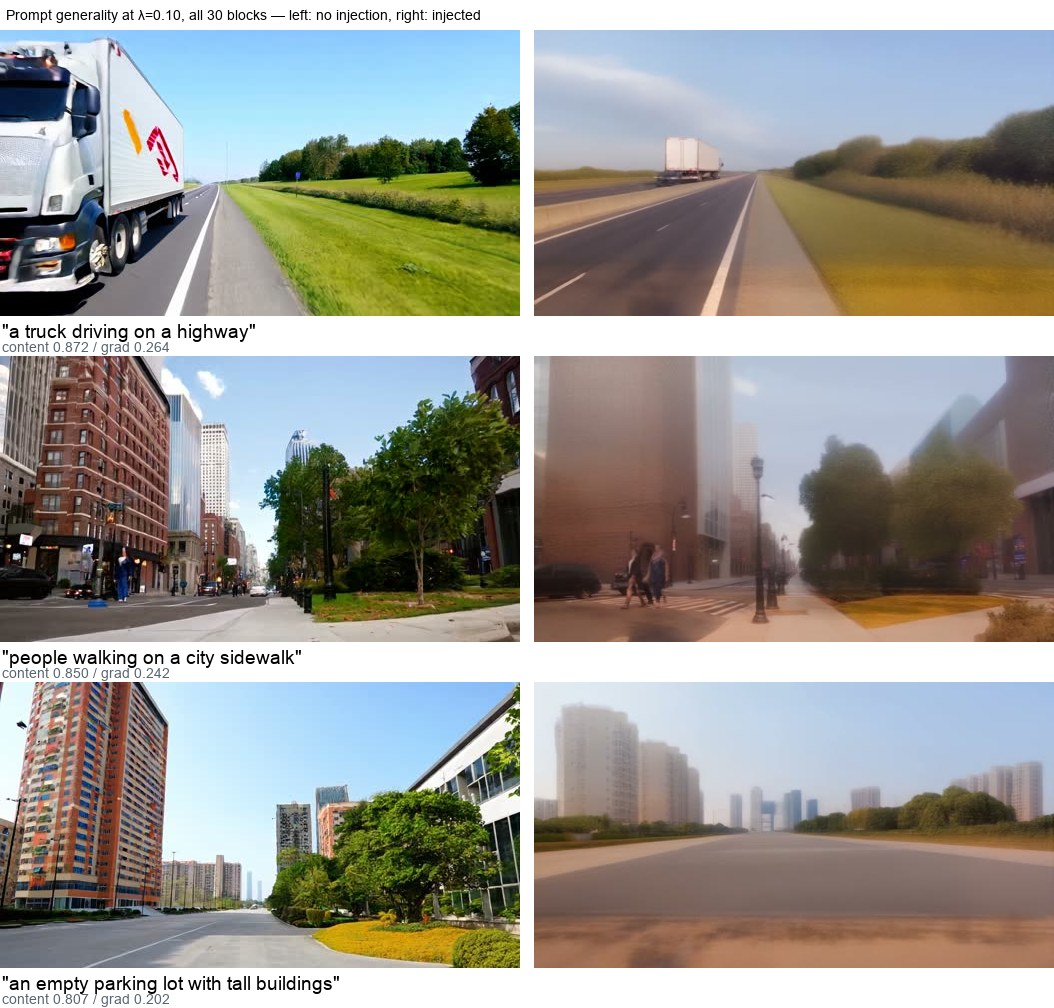
\includegraphics[width=0.48\linewidth]{figs/fig_prompt_generality.jpg}
  \caption{\textbf{Prompt generality}: $\lam{=}0.10$, all blocks, four prompts, no retuning.}
  \label{fig:prompts}
\end{figure}

\begin{figure}[!htb]
  \centering
  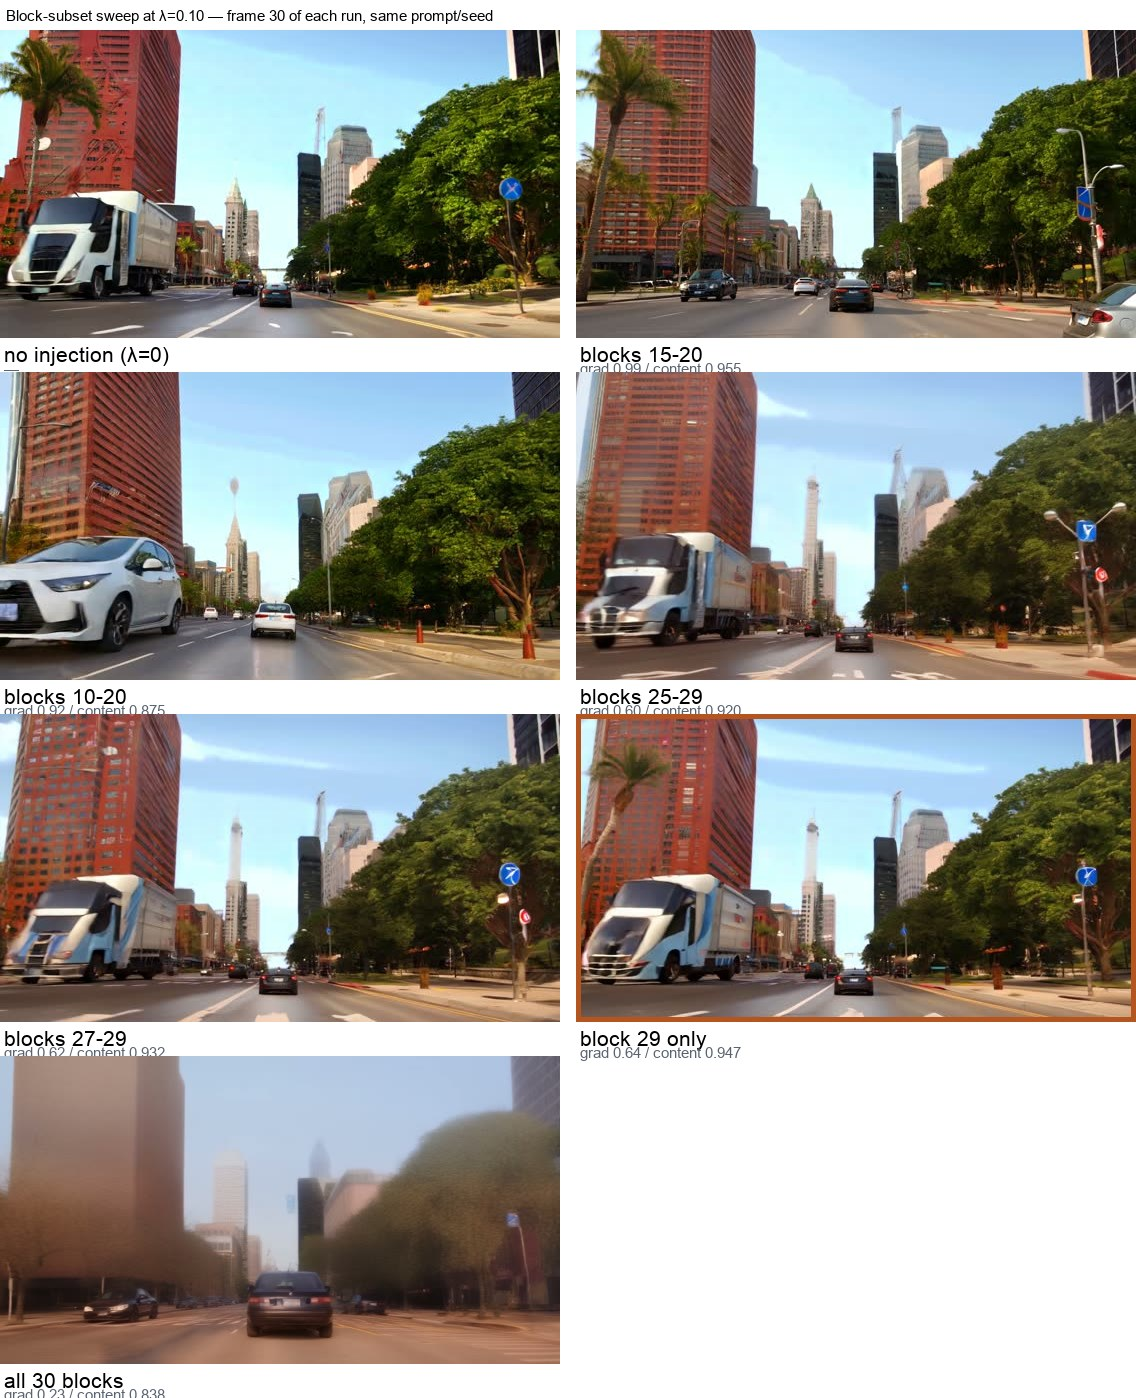
\includegraphics[width=0.48\linewidth]{figs/fig_block_subsets.jpg}
  \caption{\textbf{Block-subset injection.} No subset of up to 11 blocks produces depth-structured weather; only all 30 blocks do.}
  \label{fig:subsets}
\end{figure}

\begin{figure}[!htb]
  \centering
  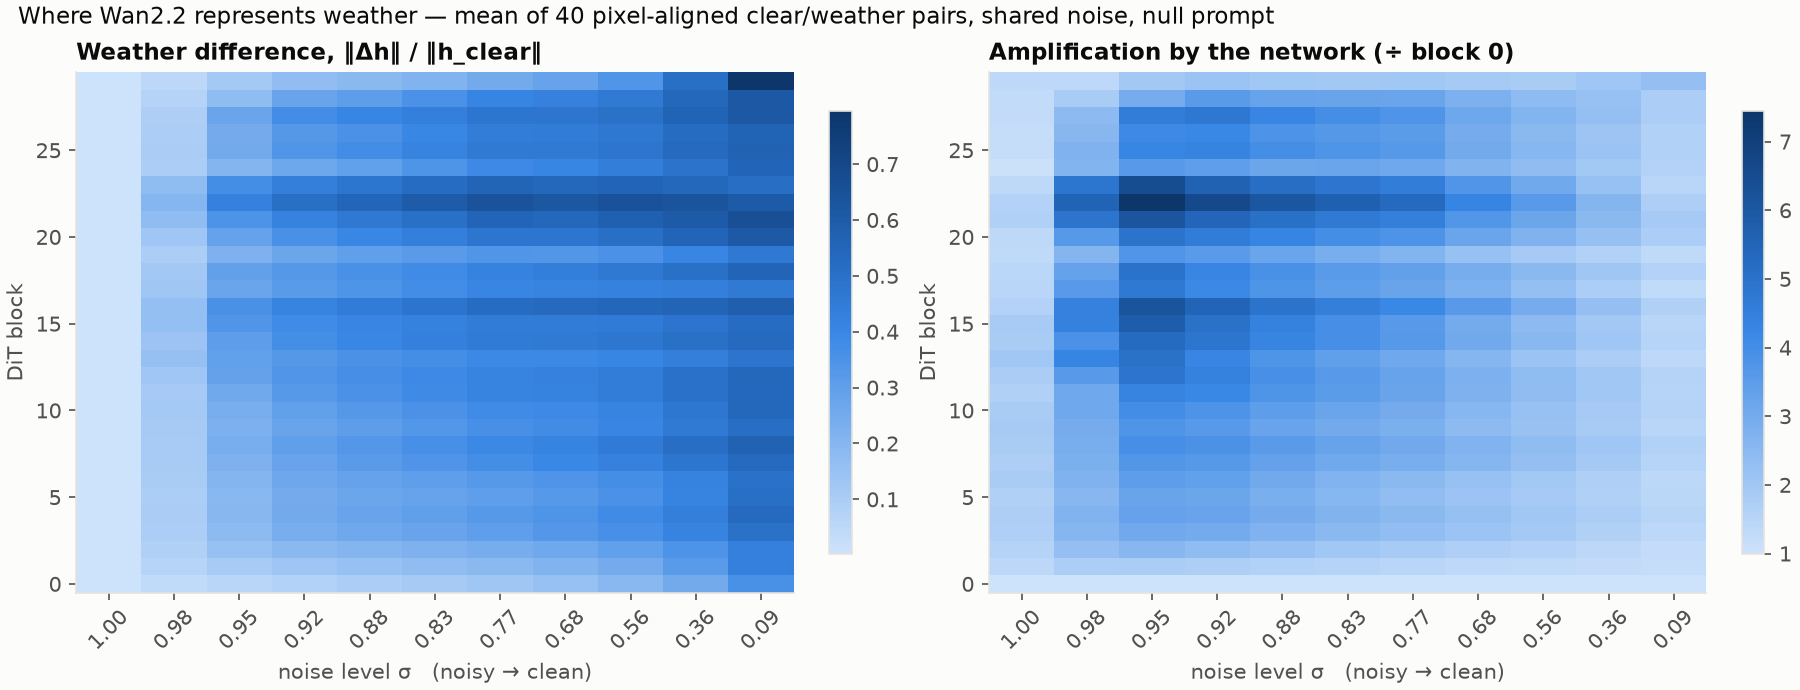
\includegraphics[width=\linewidth]{figs/fig_where.png}
  \caption{\textbf{Size of the weather difference per block and noise level} (scene 0). Left: relative to the clear activation; right: amplification relative to block 0. The block-22 peak also appears for scene differences.}
  \label{fig:where}
\end{figure}

\begin{figure}[!htb]
  \centering
  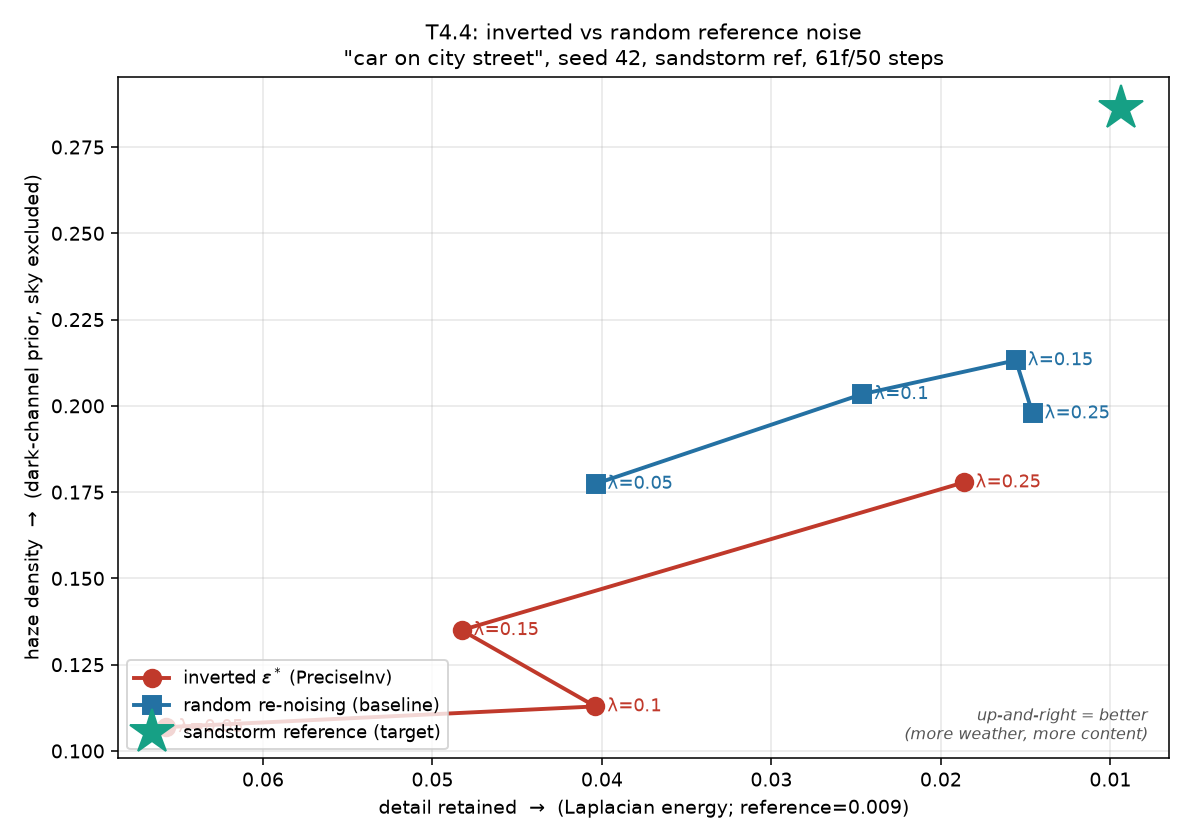
\includegraphics[width=0.62\linewidth]{figs/fig_inv_pareto.png}
  \caption{\textbf{Haze versus detail}, inverted versus random reference noise across $\lam$: every inverted point lies on or inside the random frontier.}
\end{figure}

\section{Reproducibility}
{\sloppy Code is in the project repository (branch \texttt{latent\_inspection}): \texttt{generate.py} (\texttt{--ref\_video}, \texttt{--lambda\_ref}, \texttt{--inject\_blocks}, \texttt{--inject\_sigma}, \texttt{--steer\_*}), \texttt{paired\_atlas.py} (paired probing, simulation and image modes), \texttt{paired\_inversion.py} (fixed-point inversion), \texttt{paired\_eval\_inv.py} and \texttt{paired\_eval\_kv.py} (paired ground-truth evaluation), \texttt{wan/utils/steering.py}, the analysis scripts (\texttt{analyze\_*.py}, \texttt{cross\_env.py}) and \texttt{make\_report\_figs.py}.
No model weights are modified or distributed.\par}

\end{document}
